\section{Probability and Information Theory}
\setcounter{section}{3}
%\setcounter{figure}{4}

\begin{frame}{3 Probability and Information Theory}
    \justifying
    In this chapter, we describe probability theory and information theory.
    
    Probability theory is a mathematical framework for representing uncertain statements. It provides a means of quantifying uncertainty and axioms for deriving new uncertain statements. In artificial intelligence applications, we use probability theory in two major ways. First, the laws of probability tell us how AI systems should reason, so we design our algorithms to compute or approximate various expressions derived using probability theory. Second, we can use probability and statistics to theoretically analyse the behaviour of proposed AI systems.
\end{frame}

\begin{frame}{3 Probability and Information Theory}
    \justifying
    Probability theory is a fundamental tool of many disciplines of science and engineering. We provide this chapter to ensure that readers whose background is primarily in software engineering with limited exposure to probability theory can understand the material in this book.
    
    While probability theory allows us to make uncertain statements and reason in the presence of uncertainty, information theory allows us to quantify the amount of uncertainty in a probability distribution.
\end{frame}

\begin{frame}{3 Probability and Information Theory}
    \justifying
    If you are already familiar with probability theory and information theory, you may wish to skip all of this chapter except for section 3.14 , which describes the graphs we use to describe structured probabilistic models for machine learning. If you have absolutely no prior experience with these subjects, this chapter should be sufficient to successfully carry out deep learning research projects, but we do suggest that you consult an additional resource, such as Jaynes (2003).
\end{frame}

% ======================================= Why Probability?
\subsection{Why Probability?}
\begin{frame}{3.1 Why Probability?}
    \justifying
    Many branches of computer science deal mostly with entities that are entirely deterministic and certain. A programmer can usually safely assume that a CPU will execute each machine instruction flawlessly. Errors in hardware do occur, but are rare enough that most software applications do not need to be designed to account for them. Given that many computer scientists and software engineers work in a relatively clean and certain environment, it can be surprising that machine learning makes heavy use of probability theory.
\end{frame}

\begin{frame}{3.1 Why Probability?}
    \justifying
    This is because machine learning must always deal with uncertain quantities, and sometimes may also need to deal with stochastic (non-deterministic) quantities. Uncertainty and stochasticity can arise from many sources. Researchers have made compelling arguments for quantifying uncertainty using probability since at least the 1980s. Many of the arguments presented here are summarized from or inspired by Pearl (1988).
\end{frame}

\begin{frame}{3.1 Why Probability?}
    \justifying
    Nearly all activities require some ability to reason in the presence of uncertainty. In fact, beyond mathematical statements that are true by definition, it is difficult to think of any proposition that is absolutely true or any event that is absolutely guaranteed to occur.
\end{frame}

\begin{frame}{3.1 Why Probability?}
    \justifying
    There are three possible sources of uncertainty:
    \begin{enumerate}
    \justifying
        \item Inherent stochasticity in the system being modeled. For example, most interpretations of quantum mechanics describe the dynamics of subatomic particles as being probabilistic. We can also create theoretical scenarios that we postulate to have random dynamics, such as a hypothetical card game where we assume that the cards are truly shuffled into a random order.
        \item Incomplete observability. Even deterministic systems can appear stochastic when we cannot observe all of the variables that drive the behavior of the system. For example, in the Monty Hall problem, a game show contestant is asked to choose between three doors and wins a prize held behind the chosen door. Two doors lead to a goat while a third leads to a car. The outcome given the contestant’s choice is deterministic, but from the contestant’s point of view, the outcome is uncertain.
        \seti
    \end{enumerate}
\end{frame}

\begin{frame}{3.1 Why Probability?}
    \begin{enumerate}
        \justifying
        \conti
        \item Incomplete modeling. When we use a model that must discard some of the information we have observed, the discarded information results in uncertainty in the model’s predictions. For example, suppose we build a robot that can exactly observe the location of every object around it. If the robot discretizes space when predicting the future location of these objects, then the discretization makes the robot immediately become uncertain about the precise position of objects: each object could be anywhere within the discrete cell that it was observed to occupy.
        \seti
    \end{enumerate}
\end{frame}

\begin{frame}{3.1 Why Probability?}
    \justifying
    In many cases, it is more practical to use a simple but uncertain rule rather than a complex but certain one, even if the true rule is deterministic and our modeling system has the fidelity to accommodate a complex rule. For example, the simple rule ``Most birds fly'' is cheap to develop and is broadly useful, while a rule of the form, ``Birds fly, except for very young birds that have not yet learned to fly, sick or injured birds that have lost the ability to fly, flightless species of birds including the cassowary, ostrich and kiwi...'' is expensive to develop, maintain and communicate, and after all of this effort is still very brittle and prone to failure.
\end{frame}

\begin{frame}{3.1 Why Probability?}
    \justifying
    While it should be clear that we need a means of representing and reasoning about uncertainty, it is not immediately obvious that probability theory can provide all of the tools we want for artificial intelligence applications. Probability theory was originally developed to analyze the frequencies of events. It is easy to see how probability theory can be used to study events like drawing a certain hand of cards in a game of poker. These kinds of events are often repeatable. When we say that an outcome has a probability $p$ of occurring, it means that if we repeated the experiment (e.g., draw a hand of cards) infinitely many times, then proportion $p$ of the repetitions would result in that outcome. 
\end{frame}

\begin{frame}{3.1 Why Probability?}
    \justifying
    This kind of reasoning does not seem immediately applicable to propositions that are not repeatable. If a doctor analyzes a patient and says that the patient has a $40\%$ chance of having the flu, this means something very different—we can not make infinitely many replicas of the patient, nor is there any reason to believe that different replicas of the patient would present with the same symptoms yet have varying underlying conditions. In the case of the doctor diagnosing the patient, we use probability to represent a \textbf{degree of belief}, with 1 indicating absolute certainty that the patient has the flu and 0 indicating absolute certainty that the patient does not have the flu. The former kind of probability, related directly to the rates at which events occur, is known as \textbf{frequentist probability}, while the latter, related to qualitative levels of certainty, is known as \textbf{Bayesian probability}.
\end{frame}

\begin{frame}{3.1 Why Probability?}
    \justifying
    If we list several properties that we expect common sense reasoning about uncertainty to have, then the only way to satisfy those properties is to treat Bayesian probabilities as behaving exactly the same as frequentist probabilities. For example, if we want to compute the probability that a player will win a poker game given that she has a certain set of cards, we use exactly the same formulas as when we compute the probability that a patient has a disease given that she has certain symptoms. For more details about why a small set of common sense assumptions implies that the same axioms must control both kinds of probability, see Ramsey (1926).
\end{frame}

\begin{frame}{3.1 Why Probability?}
    \justifying
    Probability can be seen as the extension of logic to deal with uncertainty. Logic provides a set of formal rules for determining what propositions are implied to be true or false given the assumption that some other set of propositions is true or false. Probability theory provides a set of formal rules for determining the likelihood of a proposition being true given the likelihood of other propositions.
\end{frame}

% ======================================= Random Variables
\subsection{Random Variables}
\begin{frame}{3.2 Random Variables}
    \justifying
    A \textbf{random variable} is a variable that can take on different values randomly. We typically denote the random variable itself with a lower case letter in plain typeface, and the values it can take on with lower case script letters. For example, $x_{1}$ and $x_{2}$ are both possible values that the random variable $\mathrm{x}$ can take on. For vector-valued variables, we would write the random variable as $\boldsymbol{\mathrm{x}}$ and one of its values as $\boldsymbol{x}$. On its own, a random variable is just a description of the states that are possible; it must be coupled with a probability distribution that specifies how likely each of these states are.
\end{frame}

\begin{frame}{3.2 Random Variables}
    \justifying
    Random variables may be discrete or continuous. A discrete random variable is one that has a finite or countably infinite number of states. Note that these states are not necessarily the integers; they can also just be named states that are not considered to have any numerical value. A continuous random variable is associated with a real value.
\end{frame}

% ======================================= Probability Distributions
\subsection{Probability Distributions}
\begin{frame}{3.3 Probability Distributions}
    \justifying
    A \textbf{probability distribution} is a description of how likely a random variable or set of random variables is to take on each of its possible states. The way we describe probability distributions depends on whether the variables are discrete or continuous.
\end{frame}

% --------------------------------------- Discrete Variables and PMF
\subsubsection{3.3.1 Discrete Variables and Probability Mass Functions}
\begin{frame}{3.3.1 Discrete Variables and Probability Mass Functions}
    \justifying
    A probability distribution over discrete variables may be described using a \textbf{Probability Mass Function} (PMF). We typically denote probability mass functions with a capital $P$. Often we associate each random variable with a different probability mass function and the reader must infer which probability mass function to use based on the identity of the random variable, rather than the name of the function; $P(\mathrm{x})$ is usually not the same as $P(\mathrm{y})$.
\end{frame}{}

\begin{frame}{3.3.1 Discrete Variables and Probability Mass Functions}
    \justifying
    The probability mass function maps from a state of a random variable to the probability of that random variable taking on that state. The probability that $\mathrm{x} = x$ is denoted as $P(x)$, with a probability of $1$ indicating that $\mathrm{x} = x$ is certain and a probability of $0$ indicating that $\mathrm{x} = x$ is impossible. Sometimes to disambiguate which PMF to use, we write the name of the random variable explicitly: $P(\mathrm{x} = x)$. Sometimes we define a variable first, then use $\sim$ notation to specify which distribution it follows later: $\mathrm{x} \sim P(\mathrm{x})$.
\end{frame}

\begin{frame}{3.3.1 Discrete Variables and Probability Mass Functions}
    \justifying
    Probability mass functions can act on many variables at the same time. Such a probability distribution over many variables is known as a \textbf{joint probability distribution}. $P(\mathrm{x} = x, \mathrm{y} = y)$ denotes the probability that $\mathrm{x} = x$ and $\mathrm{y} =y$ simultaneously. We may also write $P(x, y)$ for brevity.
\end{frame}

\begin{frame}{3.3.1 Discrete Variables and Probability Mass Functions}
    \justifying
    To be a probability mass function on a random variable $\mathrm{x}$, a function $P$ must satisfy the following properties:
    \begin{itemize}
        \justifying
        \item The domain of $P$ must be the set of all possible states of $\mathrm{x}$.
        \item $\forall x \in \mathrm{x}, 0 \leq P(x) \leq 1$. An impossible event has probability $0$ and no state can be less probable than that. Likewise, an event that is guaranteed to happen has probability $1$, and no state can have a greater chance of occurring.
        \item $\sum_{x \in \mathrm{x}} P(x) = 1$. We refer to this property as being \textbf{normalized}. Without this property, we could obtain probabilities greater than one by computing the probability of one of many events occurring.
    \end{itemize}{}
\end{frame}

\begin{frame}{3.3.1 Discrete Variables and Probability Mass Functions}
    \justifying
    For example, consider a single discrete random variable $\mathrm{x}$ with $k$ different states. We can place a \textbf{uniform distribution} on $\mathrm{x}$ -- that is, make each of its states equally likely -- by setting its probability mass function to
    \begin{equation}
        P(\mathrm{x} = x_{i}) = \frac{1}{k}
        \label{eq:3_1}
    \end{equation}
    for all $i$. We can see that this fits the requirements for a probability mass function. The value $1/k$ is positive because $k$ is a positive integer. We also see that
    \begin{equation}
        \sum_{i}P(\mathrm{x} = x_{i}) = \sum_{i}\frac{1}{k}=\frac{k}{k} = 1,
        \label{eq:3_2}
    \end{equation}
    so the distribution is properly normalized.
\end{frame}{}

% --------------------------------------- Continuous Variables and PDF
\subsubsection{3.3.2 Continuous Variables and Probability Density Functions}
\begin{frame}{3.3.2 Continuous Variables and Probability Density Functions}
    \justifying
    When working with continuous random variables, we describe probability distributions using a \textbf{Probability Density Function} (PDF) rather than a probability mass function. To be a probability density function, a function $p$ must satisfy the following properties:
    \begin{itemize}
        \justifying
        \item The domain of $p$ must be the set of all possible states of $\mathrm{x}$.
        \item $\forall x \in \mathrm{x}, p(x) \geq 0$. Note that we do not require $p(x) \leq 1$.
        \item $\int p(x) dx = 1$.
    \end{itemize}
    A probability density function $p(x)$ does not give the probability of a specific state directly, instead the probability of landing inside an infinitesimal region with volume $\delta x$ is given by $p(x)\delta x$.
\end{frame}

\begin{frame}{3.3.2 Continuous Variables and Probability Density Functions}
    \justifying
    We can integrate the density function to find the actual probability mass of a set of points. Specifically, the probability that $x$ lies in some set $\mathbb{S}$ is given by the integral of $p(x)$ over that set. In the univariate example, the probability that $x$ lies in the interval $[a, b]$ is given by $\int_{[a, b]}p(x)dx$.
\end{frame}

\begin{frame}{3.3.2 Continuous Variables and Probability Density Functions}
    \justifying
    For an example of a probability density function corresponding to a specific probability density over a continuous random variable, consider a uniform distribution on an interval of the real numbers. We can do this with a function $u(x; a, b)$, where $a$ and $b$ are the endpoints of the interval, with $b > a$. The ``$;$'' notation means ``parametrized by''; we consider $x$ to be the argument of the function, while $a$ and $b$ are parameters that define the function. To ensure that there is no probability mass outside the interval, we say $u(x; a, b) = 0$ for all $x \notin [a, b]$. Within $[a, b]$, $u(x; a, b) = \frac{1}{b - a}$. We can see that this is nonnegative everywhere. Additionally, it integrates to $1$. We often denote that $x$ follows the uniform distribution on $[a, b]$ by writing $\mathrm{x} \sim U(a, b)$.
\end{frame}

% ======================================= Marginal Probability
\subsection{Marginal Probability}
\begin{frame}{3.4 Marginal Probability}
    \justifying
    Sometimes we know the probability distribution over a set of variables and we want to know the probability distribution over just a subset of them. The probability distribution over the subset is known as the \textbf{marginal probability} distribution.
    
    For example, suppose we have discrete random variables $\mathrm{x}$ and $\mathrm{y}$, and we know $P(\mathrm{x}, \mathrm{y})$. We can find $P(\mathrm{x})$ with the \textbf{sum rule}:
    \begin{equation}
        \forall x \in \mathrm{x}, P(\mathrm{x} = x) = \sum_{y}P(\mathrm{x} = x, \mathrm{y} = y).
        \label{eq:3_3}
    \end{equation}
\end{frame}

\begin{frame}{3.4 Marginal Probability}
    \justifying
    The name ``marginal probability'' comes from the process of computing marginal probabilities on paper. When the values of $P(\mathrm{x}, \mathrm{y})$ are written in a grid with different values of $x$ in rows and different values of $y$ in columns, it is natural to sum across a row of the grid, then write $P(x)$ in the margin of the paper just to the right of the row.
    
    For continuous variables, we need to use integration instead of summation:
    \begin{equation}
        p(x) = \int p(x, y)dy.
        \label{eq:3_4}
    \end{equation}
\end{frame}

% ======================================= Conditional Probability
\subsection{Conditional Probability}
\begin{frame}{3.5 Conditional Probability}
    \justifying
    In many cases, we are interested in the probability of some event, given that some other event has happened. This is called a \textbf{conditional probability}. We denote the conditional probability that $\mathrm{y} = y$ given $\mathrm{x} = x$ as $P(\mathrm{y} = y | \mathrm{x} = x)$. This conditional probability can be computed with the formula
    \begin{equation}
        P(\mathrm{y} = y | \mathrm{x} = x) = \frac{P(\mathrm{y} = y, \mathrm{x} = x)}{P(\mathrm{x} = x)}.
        \label{eq:3_5}
    \end{equation}
    The conditional probability is only defined when $P(\mathrm{x} = x) > 0$. We cannot compute the conditional probability conditioned on an event that never happens.
\end{frame}

\begin{frame}{3.5 Conditional Probability}
    \justifying
    It is important not to confuse conditional probability with computing what would happen if some action were undertaken. The conditional probability that a person is from Germany given that they speak German is quite high, but if a randomly selected person is taught to speak German, their country of origin does not change. Computing the consequences of an action is called making an \textbf{intervention query}. Intervention queries are the domain of \textbf{causal modeling}, which we do not explore in this book.
\end{frame}{}

% ======================================= The Chain Rule of Conditional Probabilities
\subsection{The Chain Rule of Conditional Probabilities}
\begin{frame}{3.6 The Chain Rule of Conditional Probabilities}
    \justifying
    Any joint probability distribution over many random variables may be decomposed into conditional distributions over only one variable:
    \begin{equation}
        P(\mathrm{x}^{(1)}, ..., \mathrm{x}^{(n)}) = P(\mathrm{x}^{(1)})\prod^{n}_{i = 2} P(\mathrm{x}^{(i)} | \mathrm{x}^{(1)}, ..., \mathrm{x}^{(i-1)}).
        \label{eq:3_6}
    \end{equation}
    This observation is known as the chain rule or product rule of probability. It follows immediately from the definition of conditional probability in equation \ref{eq:3_5}.
\end{frame}

\begin{frame}{3.6 The Chain Rule of Conditional Probabilities}
    For example, applying the definition twice, we get
    \begin{align}
        P(\mathrm{a}, \mathrm{b}, \mathrm{c}) &= P(\mathrm{a} | \mathrm{b}, \mathrm{c}) P(\mathrm{b}, \mathrm{c}) \nonumber\\
        P(\mathrm{b}, \mathrm{c}) &= P(\mathrm{b} | \mathrm{c}) P(\mathrm{c}) \nonumber\\
        P(\mathrm{a}, \mathrm{b}, \mathrm{c}) &= P(\mathrm{a} | \mathrm{b}, \mathrm{c}) P(\mathrm{b} | \mathrm{c}) P(\mathrm{c}) \nonumber
    \end{align}
\end{frame}

% ======================================= Independence and Conditional Independence
\subsection{Independence and Conditional Independence}
\begin{frame}{3.7 Independence and Conditional Independence}
    \justifying
    Two random variables $\mathrm{x}$ and $\mathrm{y}$ are \textbf{independent} if their probability distribution can be expressed as a product of two factors, one involving only $\mathrm{x}$ and one involving only $\mathrm{y}$:
    \begin{equation}
        \forall x \in \mathrm{x}, y \in \mathrm{y}, p(\mathrm{x} = x, \mathrm{y} = y) = p(\mathrm{x} = x) p(\mathrm{y} = y).
        \label{eq:3_7}
    \end{equation}
\end{frame}

\begin{frame}{3.7 Independence and Conditional Independence}
    \justifying
    Two random variables $\mathrm{x}$ and $\mathrm{y}$ are \textbf{conditionally independent} given a random variable $\mathrm{z}$ if the conditional probability distribution over $\mathrm{x}$ and $\mathrm{y}$ factorizes in this way for every value of $\mathrm{z}$:
    \begin{align}
        \forall x \in \mathrm{x}, y \in \mathrm{y},  \in \mathrm{z}, &\nonumber \\ 
        p(\mathrm{x} = x, \mathrm{y} = y | \mathrm{z} = z) &= p(\mathrm{x} = x | \mathrm{z} = z) p(\mathrm{y} = y | \mathrm{z} = z).
        \label{eq:3_8}    
    \end{align}
    We can denote independence and conditional independence with compact notation: $\mathrm{x} \perp \mathrm{y}$ means that $\mathrm{x}$ and $\mathrm{y}$ are independent, while $\mathrm{x} \perp \mathrm{y} | \mathrm{z}$ means that $\mathrm{x}$ and $\mathrm{y}$ are conditionally independent given $\mathrm{z}$.
\end{frame}

% ======================================= Expectation, Variance and Covariance
\subsection{Expectation, Variance and Covariance}
\begin{frame}{3.8 Expectation, Variance and Covariance}
    \justifying
    The \textbf{expectation} or \textbf{expected value} of some function $f(x)$ with respect to a probability distribution $P(\mathrm{x})$ is the average or mean value that $f$ takes on when $x$ is drawn from $P$. For discrete variables this can be computed with a summation:
    \begin{equation}
        \mathbb{E}_{\mathrm{x} \sim P}[f(x)] = \sum_{x} P(x) f(x),
        \label{eq:3_9}
    \end{equation}
    while for continuous variable, it is computed with an integral:
    \begin{equation}
        \mathbb{E}_{\mathrm{x} \sim p}[f(x)] = \int p(x) f(x)dx,
        \label{eq:3_10}
    \end{equation}
\end{frame}{}

\begin{frame}{3.8 Expectation, Variance and Covariance}
    \justifying
    When the identity of the distribution is clear from the context, we may simply write the name of the random variable that the expectation is over, as in $\mathbb{E}_{\mathrm{x}}[f(x)]$. If it is clear which random variable the expectation is over, we may omit the subscript entirely, as in $\mathbb{E}[f(x)]$. By default, we can assume that $\mathbb{E}[\cdot]$ averages over the values of all the random variables inside the brackets. Likewise, when there is no ambiguity, we may omit the square brackets.
    
    Expectations are linear, for example,
    \begin{equation}
        \mathbb{E}_{\mathrm{x}}[\alpha f(x) + \beta g(x)] = \alpha\mathbb{E}_{\mathrm{x}}[f(x)] + \beta\mathbb{E}_{\mathrm{x}}[g(x)],
        \label{eq:3_11}
    \end{equation}
    when $\alpha$ and $\beta$ are not dependent on $x$.
\end{frame}

\begin{frame}{3.8 Expectation, Variance and Covariance}
    \justifying
    The \textbf{variance} gives a measure of how much the values of a function of a random variable $\mathrm{x}$ vary as we sample different values of $x$ from its probability distribution:
    \begin{equation}
        Var(f(x)) = \mathbb{E}[\,(f(x) - \mathbb{E}[f(x)])^{2}]\,.
        \label{eq:3_12}
    \end{equation}
    
    When the variance is low, the values of $f(x)$ cluster near their expected value. The square root of the variance is known as the \textbf{standard deviation}.
\end{frame}

\begin{frame}{3.8 Expectation, Variance and Covariance}
    \justifying
    The \textbf{covariance} gives some sense of how much two values are linearly related to each other, as well as the scale of these variables:
    \begin{equation}
        Cov(f(x), g(y)) = \mathbb{E}[\,(f(x) - \mathbb{E}[f(x)]) (g(y) - \mathbb{E}[g(y)])]\,.
        \label{eq:3_13}
    \end{equation}
    High absolute values of the covariance mean that the values change very much and are both far from their respective means at the same time. If the sign of the covariance is positive, then both variables tend to take on relatively high values simultaneously. If the sign of the covariance is negative, then one variable tends to take on a relatively high value at the times that the other takes on a relatively low value and vice versa. Other measures such as \textbf{correlation} normalize the contribution of each variable in order to measure only how much the variables are related, rather than also being affected by the scale of the separate variables.
\end{frame}

\begin{frame}{3.8 Expectation, Variance and Covariance}
    \justifying
    The notions of covariance and dependence are related, but are in fact distinct concepts. They are related because two variables that are independent have zero covariance, and two variables that have non-zero covariance are dependent. However, independence is a distinct property from covariance. For two variables to have zero covariance, there must be no linear dependence between them. Independence is a stronger requirement than zero covariance, because independence also excludes nonlinear relationships. It is possible for two variables to be dependent but have zero covariance.
\end{frame}

\begin{frame}{3.8 Expectation, Variance and Covariance}
    \justifying
    For example, suppose we first sample a real number $x$ from a uniform distribution over the interval $[−1, 1]$. We next sample a random variable $s$. With probability $\frac{1}{2}$, we choose the value of $s$ to be $1$. Otherwise, we choose the value of $s$ to be $−1$. We can then generate a random variable $y$ by assigning $y = sx$. Clearly, $x$ and $y$ are not independent, because $x$ completely determines the magnitude of $y$. However, $Cov(x, y) = 0$.
\end{frame}

\begin{frame}{3.8 Expectation, Variance and Covariance}
    \justifying    
    The \textbf{covariance matrix} of a random vector $\boldsymbol{x} \in \mathbb{R}^{n}$ is an $n \times n$ matrix, such that
    \begin{equation}
        Cov(\boldsymbol{\mathrm{x}})_{i, j} = Cov(\mathrm{x}_{i}, \mathrm{x}_{j}).
        \label{eq:3_14}
    \end{equation}
    
    The diagonal elements of the covariance give the variance:
    \begin{equation}
        Cov(\mathrm{x}_{i}, \mathrm{x}_{j}) = Var(\mathrm{x}_{i}).
        \label{eq:3_15}
    \end{equation}{}
\end{frame}


% ======================================= Common Probability Distributions
\subsection{Common Probability Distributions}
\begin{frame}{3.9 Common Probability Distributions}
    \justifying
    Several simple probability distributions are useful in many contexts in machine learning.
\end{frame}

% --------------------------------------- Bernoulli Distribution
\subsubsection{3.9.1 Bernoulli Distribution}
\begin{frame}{3.9.1 Bernoulli Distribution}
    \justifying
    The \textbf{Bernoulli} distribution is a distribution over a single binary random variable. It is controlled by a single parameter $\phi \in  [0, 1]$, which gives the probability of the random variable being equal to $1$. It has the following properties:
    \begin{align}
        P(\mathrm{x} = 1) &= \phi \label{eq:3_16}\\
        P(\mathrm{x} = 0) &= 1 - \phi \label{eq:3_17}\\
        P(\mathrm{x} = x) &= \phi^{x}(1 - \phi)^{1 - x} \label{eq:3_18}\\
        \mathbb{E}_{\mathrm{x}}[\mathrm{x}] &= \phi \label{eq:3_19}\\
        Var_{\mathrm{x}}(\mathrm{x}) &= \phi(1 - \phi) \label{eq:3_20}
    \end{align}
\end{frame}

% --------------------------------------- Multinoulli Distribution
\subsubsection{3.9.2 Multinoulli Distribution}
\begin{frame}{3.9.2 Multinoulli Distribution}
    \justifying
    The \textbf{multinoulli} or \textbf{categorical} distribution is a distribution over a single discrete variable with $k$ different states, where $k$ is finite (nota de rodap\'{e} aqui!). The multinoulli distribution is parametrized by a vector $\boldsymbol{p} \in [0, 1]^{k−1}$, where $p_{i}$ gives the probability of the $i$-th state. The final, $k$-th state’s probability is given by $1 − \boldsymbol{1}^{T}\boldsymbol{p}$. Note that we must constrain $\boldsymbol{1}^{T} \boldsymbol{p} \leq 1$. Multinoulli distributions are often used to refer to distributions over categories of objects, so we do not usually assume that state $1$ has numerical value $1$, etc. For this reason, we do not usually need to compute the expectation or variance of multinoulli-distributed random variables.
\end{frame}

\begin{frame}{3.9.2 Multinoulli Distribution}
    \justifying
    The Bernoulli and multinoulli distributions are sufficient to describe any distribution over their domain. They are able to describe any distribution over their domain not so much because they are particularly powerful but rather because their domain is simple; they model discrete variables for which it is feasible to enumerate all of the states. When dealing with continuous variables, there are uncountably many states, so any distribution described by a small number of parameters must impose strict limits on the distribution.
\end{frame}

% --------------------------------------- Gaussian Distribution
\subsubsection{3.9.3 Gaussian Distribution}
\begin{frame}{3.9.3 Gaussian Distribution}
    \justifying
    The most commonly used distribution over real numbers is the \textbf{normal distribution}, also known as the \textbf{Gaussian distribution}:
    \begin{equation}
        \mathcal{N}(x; \mu, \sigma^{2}) = \sqrt{\frac{1}{2\pi\sigma^{2}}} \exp\left(-\frac{1}{2\sigma^{2}} (x - \mu)^{2}\right).
        \label{eq:3_21}
    \end{equation}
    
    See figure~3.1(\ref{fig:3_1the_normal_distribution}) for a plot of the density function.
    
    The two parameters $\mu \in \mathbb{R}$ and $\sigma \in (0, ∞)$ control the normal distribution. The parameter $\mu$ gives the coordinate of the central peak. This is also the mean of the distribution: $\mathbb{E}[\mathrm{x}] = \mu$. The standard deviation of the distribution is given by $\sigma$, and the variance by $\sigma^{2}$.
\end{frame}

\begin{frame}{3.9.3 Gaussian Distribution}
    \begin{figure}
        \centering
        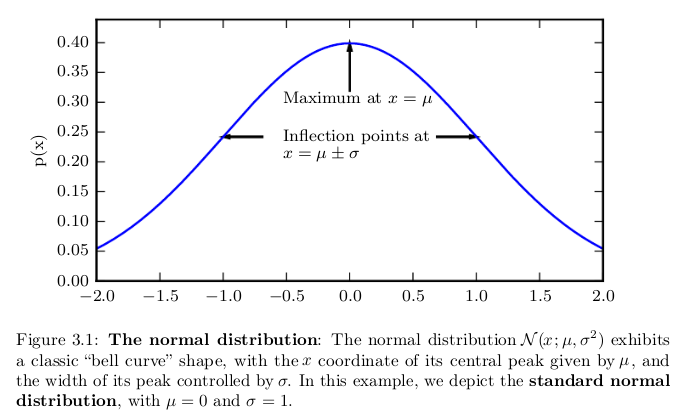
\includegraphics[scale=0.45]{images/3-1-gaussian_distribution.png}
        \label{fig:3_1the_normal_distribution}
        \caption{\textbf{The normal distribution}}
    \end{figure}
\end{frame}

\begin{frame}{3.9.3 Gaussian Distribution}
    \justifying
    When we evaluate the PDF, we need to square and invert $\sigma$. When we need to frequently evaluate the PDF with different parameter values, a more efficient way of parametrizing the distribution is to use a parameter $\beta \in (0, ∞)$ to control the precision or inverse variance of the distribution:
    \begin{equation}
        \mathcal{N}(x; \mu, \beta^{-1}) = \sqrt{\frac{\beta}{2\pi}} \exp\left(-\frac{1}{2} \beta (x - \mu)^{2}\right).
        \label{eq:3_22}
    \end{equation}
    
    Normal distributions are a sensible choice for many applications. In the absence of prior knowledge about what form a distribution over the real numbers should take, the normal distribution is a good default choice for two major reasons.
\end{frame}

\begin{frame}{3.9.3 Gaussian Distribution}
    \justifying
    First, many distributions we wish to model are truly close to being normal distributions. The \textbf{central limit theorem} shows that the sum of many independent random variables is approximately normally distributed. This means that in practice, many complicated systems can be modeled successfully as normally distributed noise, even if the system can be decomposed into parts with more structured behavior.
\end{frame}

\begin{frame}{3.9.3 Gaussian Distribution}
    \justifying
    Second, out of all possible probability distributions with the same variance, the normal distribution encodes the maximum amount of uncertainty over the real numbers. We can thus think of the normal distribution as being the one that inserts the least amount of prior knowledge into a model. Fully developing and justifying this idea requires more mathematical tools, and is postponed to section 19.4.2.
\end{frame}

\begin{frame}{3.9.3 Gaussian Distribution}
    \justifying
    The normal distribution generalizes to $\mathbb{R}^{n}$, in which case it is known as the \textbf{multivariate normal distribution}. It may be parametrized with a positive definite symmetric matrix $\boldsymbol{\Sigma}$:
    \begin{equation}
        \mathcal{N}(\boldsymbol{x}; \boldsymbol{\mu}, \boldsymbol{\Sigma}) = \sqrt{\frac{1}{(2 \pi)^{n} \det(\boldsymbol{\Sigma})}} \exp\left(-\frac{1}{2}(\boldsymbol{x} - \boldsymbol{\mu})^{T} \boldsymbol{\Sigma}^{-1} (\boldsymbol{x} - \boldsymbol{\mu})\right).
        \label{eq:3_23}
    \end{equation}
\end{frame}

\begin{frame}{3.9.3 Gaussian Distribution}
    \justifying
    The parameter $\boldsymbol{\mu}$ still gives the mean of the distribution, though now it is vector-valued. The parameter $\boldsymbol{\Sigma}$ gives the covariance matrix of the distribution. As in the univariate case, when we wish to evaluate the PDF several times for many different values of the parameters, the covariance is not a computationally efficient way to parametrize the distribution, since we need to invert $\boldsymbol{\Sigma}$ to evaluate the PDF. We can instead use a \textbf{precision matrix} $\boldsymbol{\beta}$:
    \begin{equation}
        \mathcal{N}(\boldsymbol{x}; \boldsymbol{\mu}, \boldsymbol{\beta}^{-1}) = \sqrt{\frac{\det(\boldsymbol{\beta})}{(2 \pi)^{n}}} \exp\left(-\frac{1}{2}(\boldsymbol{x} - \boldsymbol{\mu})^{T} \boldsymbol{\beta} (\boldsymbol{x} - \boldsymbol{\mu})\right).        
        \label{eq:3_24}
    \end{equation}
    
    We often fix the covariance matrix to be a diagonal matrix. An even simpler version is the \textbf{isotropic} Gaussian distribution, whose covariance matrix is a scalar times the identity matrix.
\end{frame}

% --------------------------------------- Exponential and Laplace Distributions
\subsubsection{3.9.4 Exponential and Laplace Distributions}
\begin{frame}{3.9.4 Exponential and Laplace Distributions}
    \justifying
    In the context of deep learning, we often want to have a probability distribution with a sharp point at $x = 0$. To accomplish this, we can use the \textbf{exponential distribution}:
    \begin{equation}
        p(x; \lambda) = \lambda\boldsymbol{1}_{x\geq0}\exp(-\lambda x).
        \label{eq:3_25}
    \end{equation}
    
    The exponential distribution uses the indicator function $\boldsymbol{1}_{x\geq0}$ to assign probability zero to all negative values of $x$.
\end{frame}

\begin{frame}{3.9.4 Exponential and Laplace Distributions}
    \justifying
    A closely related probability distribution that allows us to place a sharp peak of probability mass at an arbitrary point $\mu$ is the \textbf{Laplace distribution}
    \begin{equation}
        Laplace(x; \mu, \gamma) = \frac{1}{2\gamma}\exp\left(-\frac{|x - \mu|}{\gamma} \right).
        \label{eq:3_26}
    \end{equation}
\end{frame}

% --------------------------------------- The Dirac Distribution and Empirical Distribution
\subsubsection{3.9.5 The Dirac Distribution and Empirical Distribution}
\begin{frame}{3.9.5 The Dirac Distribution and Empirical Distribution}
    \justifying
    In some cases, we wish to specify that all of the mass in a probability distribution clusters around a single point. This can be accomplished by defining a PDF using the Dirac delta function, $\delta(x)$:
    \begin{equation}
        p(x) = \delta(x - \mu).
        \label{eq:3_27}
    \end{equation}
    
    The Dirac delta function is defined such that it is zero-valued everywhere except $0$, yet integrates to $1$. The Dirac delta function is not an ordinary function that associates each value $x$ with a real-valued output, instead it is a different kind of mathematical object called a \textbf{generalized function} that is defined in terms of its properties when integrated. We can think of the Dirac delta function as being the limit point of a series of functions that put less and less mass on all points other than zero.
\end{frame}

\begin{frame}{3.9.5 The Dirac Distribution and Empirical Distribution}
    \justifying
    By defining $p(x)$ to be $\delta$ shifted by $−\mu$ we obtain an infinitely narrow and infinitely high peak of probability mass where $x = \mu$. A common use of the Dirac delta distribution is as a component of an \textbf{empirical distribution},
    \begin{equation}
        \hat{p}(\boldsymbol{x}) = \frac{1}{m}\sum^{m}_{i = 1} \delta(\boldsymbol{x} - \boldsymbol{x}^{(i)})
        \label{eq:3_28}
    \end{equation}
    which puts probability mass $\frac{1}{m}$ on each of the $m$ points $\boldsymbol{x}^{(1)}, ..., \boldsymbol{x}^{(m)}$ forming a given dataset or collection of samples. The Dirac delta distribution is only necessary to define the empirical distribution over continuous variables. For discrete variables, the situation is simpler: an empirical distribution can be conceptualized as a multinoulli distribution, with a probability associated to each possible input value that is simply equal to the \textbf{empirical frequency} of that value in the training set.
\end{frame}

\begin{frame}{3.9.5 The Dirac Distribution and Empirical Distribution}
    \justifying
    We can view the empirical distribution formed from a dataset of training examples as specifying the distribution that we sample from when we train a model on this dataset. Another important perspective on the empirical distribution is that it is the probability density that maximizes the likelihood of the training data (see section 5.5).
\end{frame}

% --------------------------------------- Mixture of Distributions
\subsubsection{3.9.6 Mixture of Distributions}
\begin{frame}{3.9.6 Mixture of Distributions}
    \justifying
    It is also common to define probability distributions by combining other simpler probability distributions. One common way of combining distributions is to construct a \textbf{mixture distribution}. A mixture distribution is made up of several component distributions. On each trial, the choice of which component distribution generates the sample is determined by sampling a component identity from a multinoulli distribution:
    \begin{equation}
        P(\mathrm{x}) = \sum_{i} P(\mathrm{c} = i) P(\mathrm{x} | \mathrm{c} = i)
        \label{eq:3_29}
    \end{equation}
    where $P(\mathrm{c})$ is the multinoulli distribution over component identities.
\end{frame}

\begin{frame}{3.9.6 Mixture of Distributions}
    \justifying
    We have already seen one example of a mixture distribution: the empirical distribution over real-valued variables is a mixture distribution with one Dirac component for each training example.
    
    The mixture model is one simple strategy for combining probability distributions to create a richer distribution. In chapter 16, we explore the art of building complex probability distributions from simple ones in more detail.
\end{frame}

\begin{frame}{3.9.6 Mixture of Distributions}
    \justifying
    The mixture model allows us to briefly glimpse a concept that will be of paramount importance later -- the \textbf{latent variable}. A latent variable is a random variable that we cannot observe directly. The component identity variable c of the mixture model provides an example. Latent variables may be related to x through the joint distribution, in this case, $P(\mathrm{x}, \mathrm{c}) = P(\mathrm{x} | \mathrm{c})P(\mathrm{c})$. The distribution $P(\mathrm{c})$ over the latent variable and the distribution $P(\mathrm{x} | \mathrm{c})$ relating the latent variables to the visible variables determines the shape of the distribution $P(\mathrm{x})$ even though it is possible to describe $P(\mathrm{x})$ without reference to the latent variable. Latent variables are discussed further in section 16.5.
\end{frame}

\begin{frame}{3.9.6 Mixture of Distributions}
    \justifying
    A very powerful and common type of mixture model is the \textbf{Gaussian mixture} model, in which the components $p(\boldsymbol{\mathrm{x}} | \mathrm{c} = i)$ are Gaussians. Each component has a separately parametrized mean $\boldsymbol{\mu}^{(i)}$ and covariance $\boldsymbol{\Sigma}^{(i)}$. Some mixtures can have more constraints. For example, the covariances could be shared across components via the constraint $\boldsymbol{\Sigma}^{(i)} = \boldsymbol{\Sigma}, \forall i$. As with a single Gaussian distribution, the mixture of Gaussians might constrain the covariance matrix for each component to be diagonal or isotropic.
\end{frame}

\begin{frame}{3.9.6 Mixture of Distributions}
    \justifying
    In addition to the means and covariances, the parameters of a Gaussian mixture specify the \textbf{prior probability} $\alpha_{i} = P(\mathrm{c} = i)$ given to each component $i$. The word ``prior'' indicates that it expresses the model’s beliefs about $\mathrm{c}$ \textit{before} it has observed $\boldsymbol{\mathrm{x}}$. By comparison, $P(\mathrm{c} | \boldsymbol{\mathrm{x}})$ is a \textbf{posterior probability}, because it is computed after observation of $\boldsymbol{\mathrm{x}}$. A Gaussian mixture model is a \textbf{universal approximator} of densities, in the sense that any smooth density can be approximated with any specific, non-zero amount of error by a Gaussian mixture model with enough components.
    
    Figure~3.2(\ref{fig:3_2gaussian_mixture}) shows samples from a Gaussian mixture model.
\end{frame}

\begin{frame}{3.9.6 Mixture of Distributions}
    \begin{figure}
        \centering
        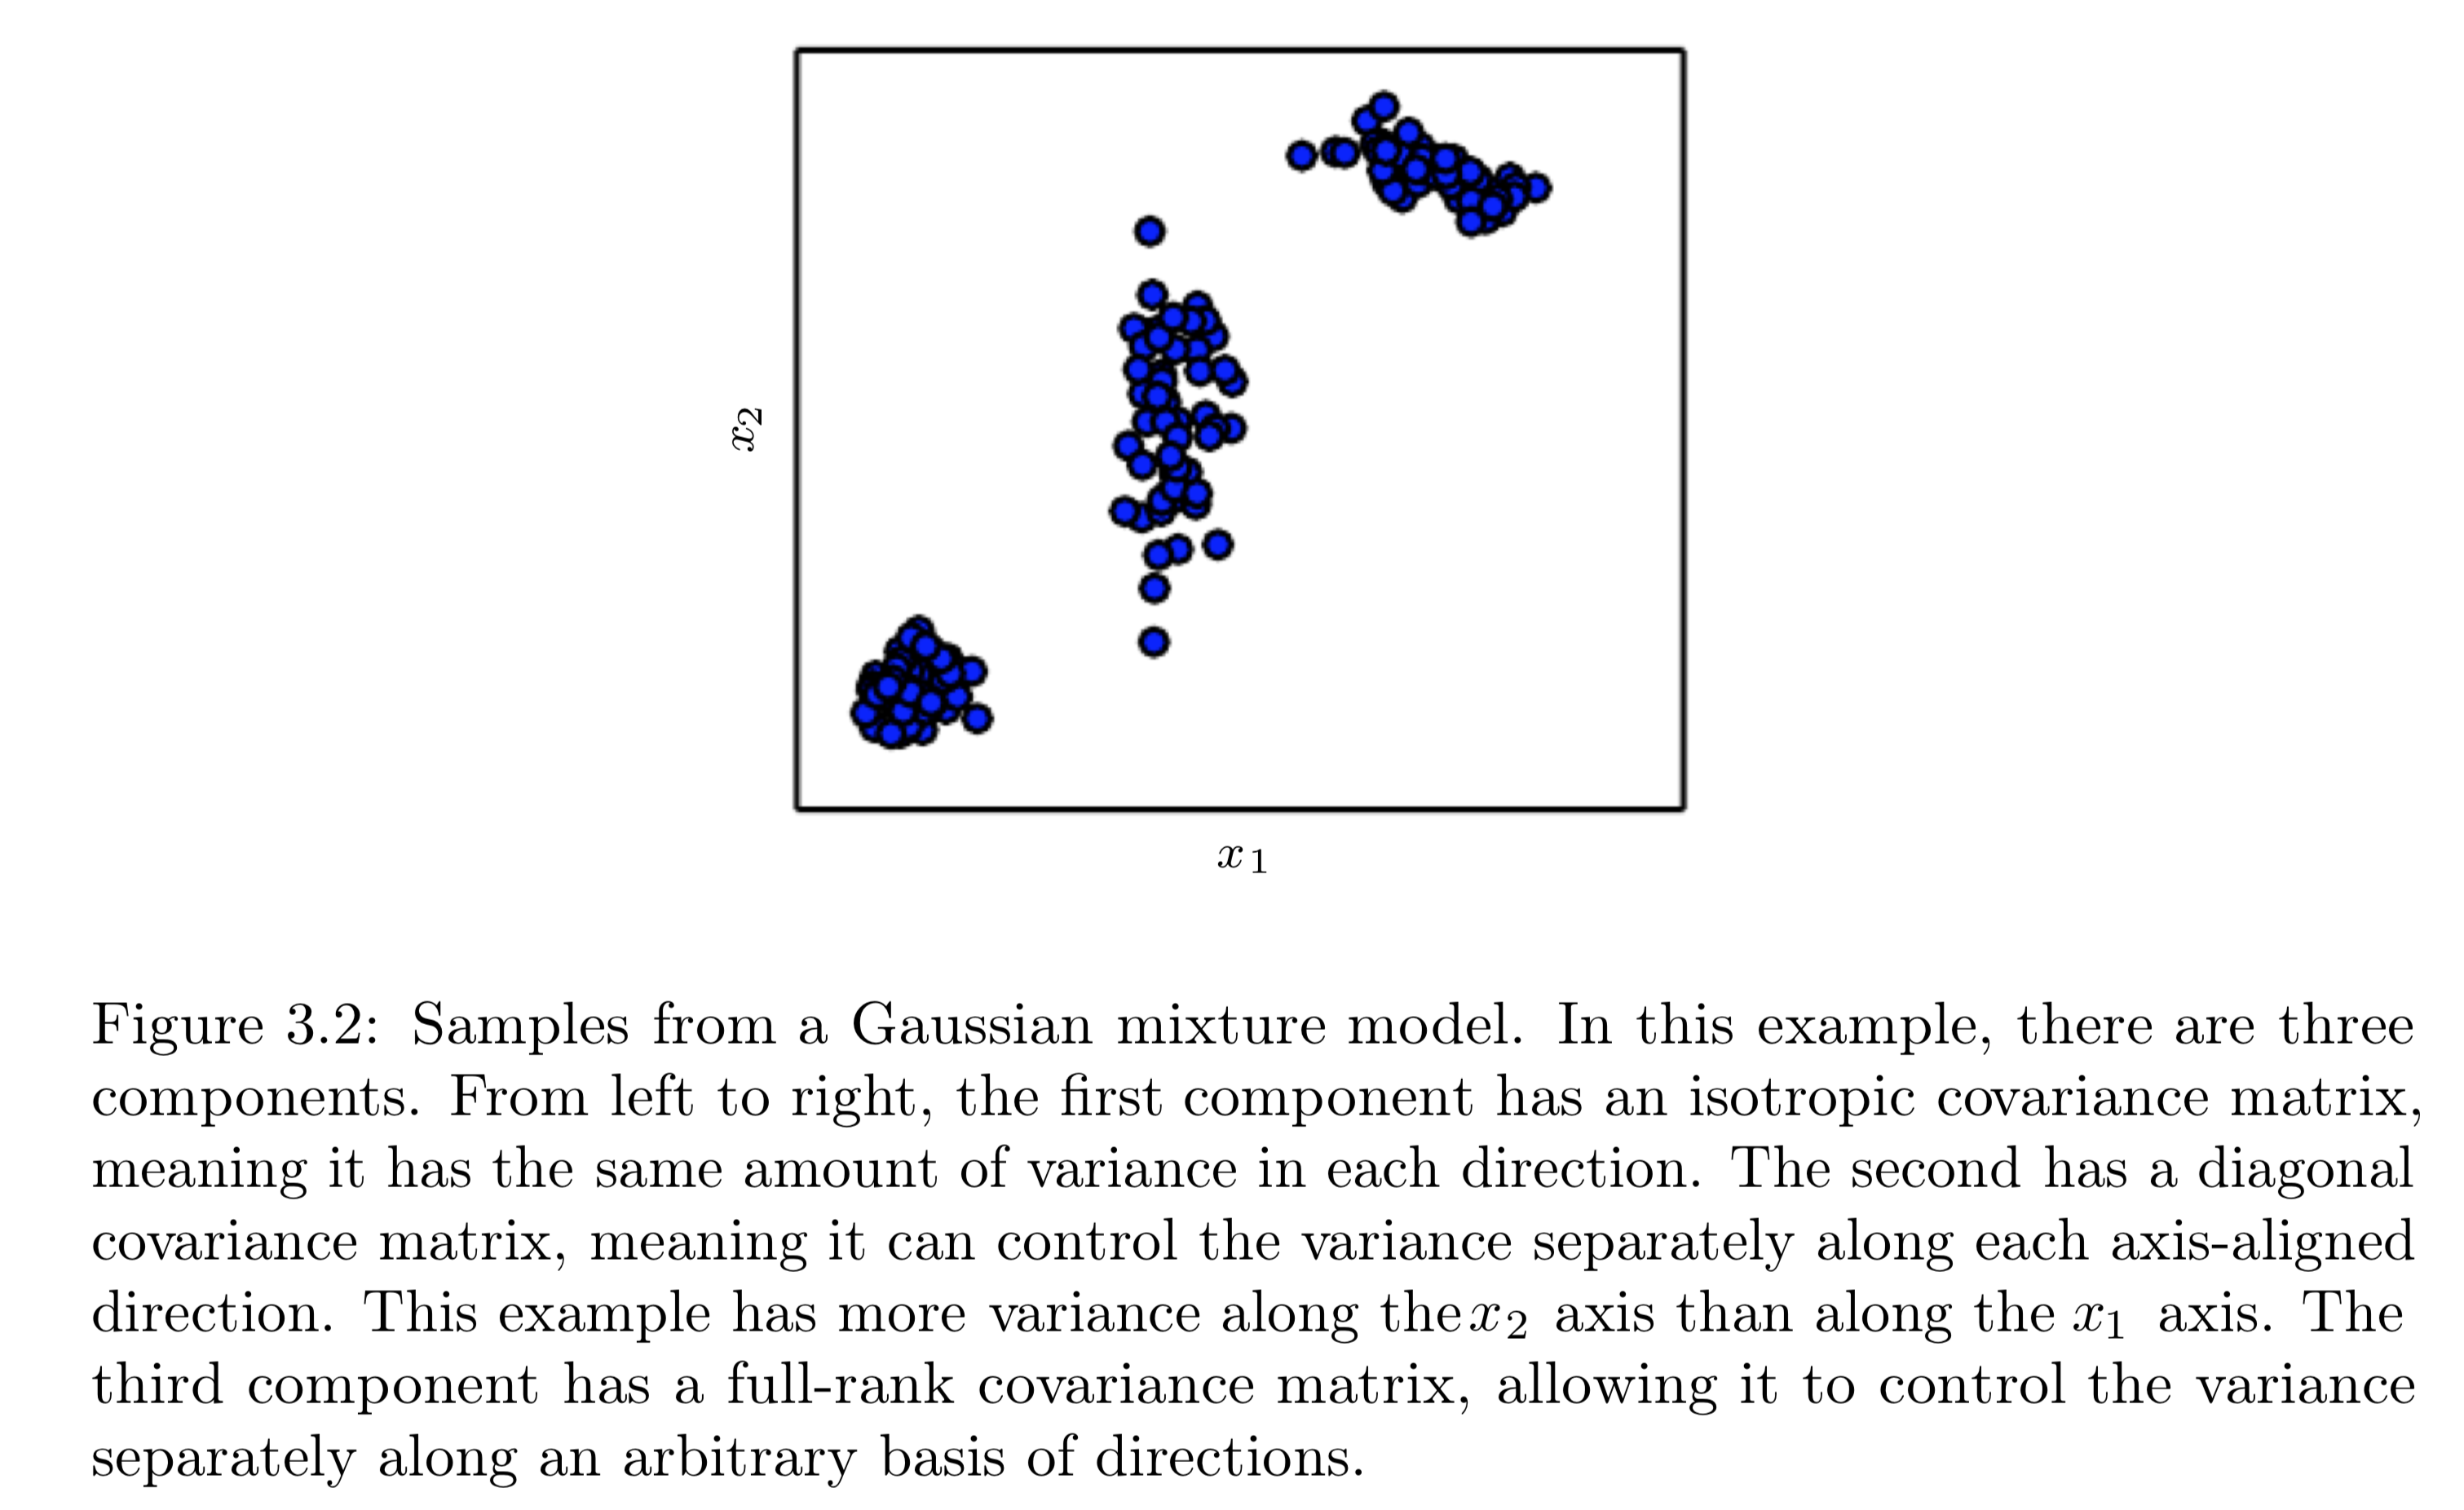
\includegraphics[scale=0.20]{images/3-2-gaussian_mixture.png}
        \label{fig:3_2gaussian_mixture}
        \caption{\textbf{The gaussian mixture}}
    \end{figure}
\end{frame}

% ======================================= Useful Properties of Common Functions
\subsection{Useful Properties of Common Functions}
\begin{frame}{3.10 Useful Properties of Common Functions}
    \justifying
    Certain functions arise often while working with probability distributions, especially the probability distributions used in deep learning models.
    
    One of these functions is the \textbf{logistic sigmoid}:
    \begin{equation}
        \sigma(x) = \frac{1}{1 + \exp(-x)}.
        \label{eq:3_30}
    \end{equation}
    
    The logistic sigmoid is commonly used to produce the $\phi$ parameter of a Bernoulli distribution because its range is $(0, 1)$, which lies within the valid range of values for the $\phi$ parameter. See figure~3.3(\ref{fig:3_3sigmoid}) for a graph of the sigmoid function. The sigmoid function \textbf{saturates} when its argument is very positive or very negative, meaning that the function becomes very flat and insensitive to small changes in its input.
\end{frame}

\begin{frame}{3.10 Useful Properties of Common Functions}
    \begin{figure}
        \centering
        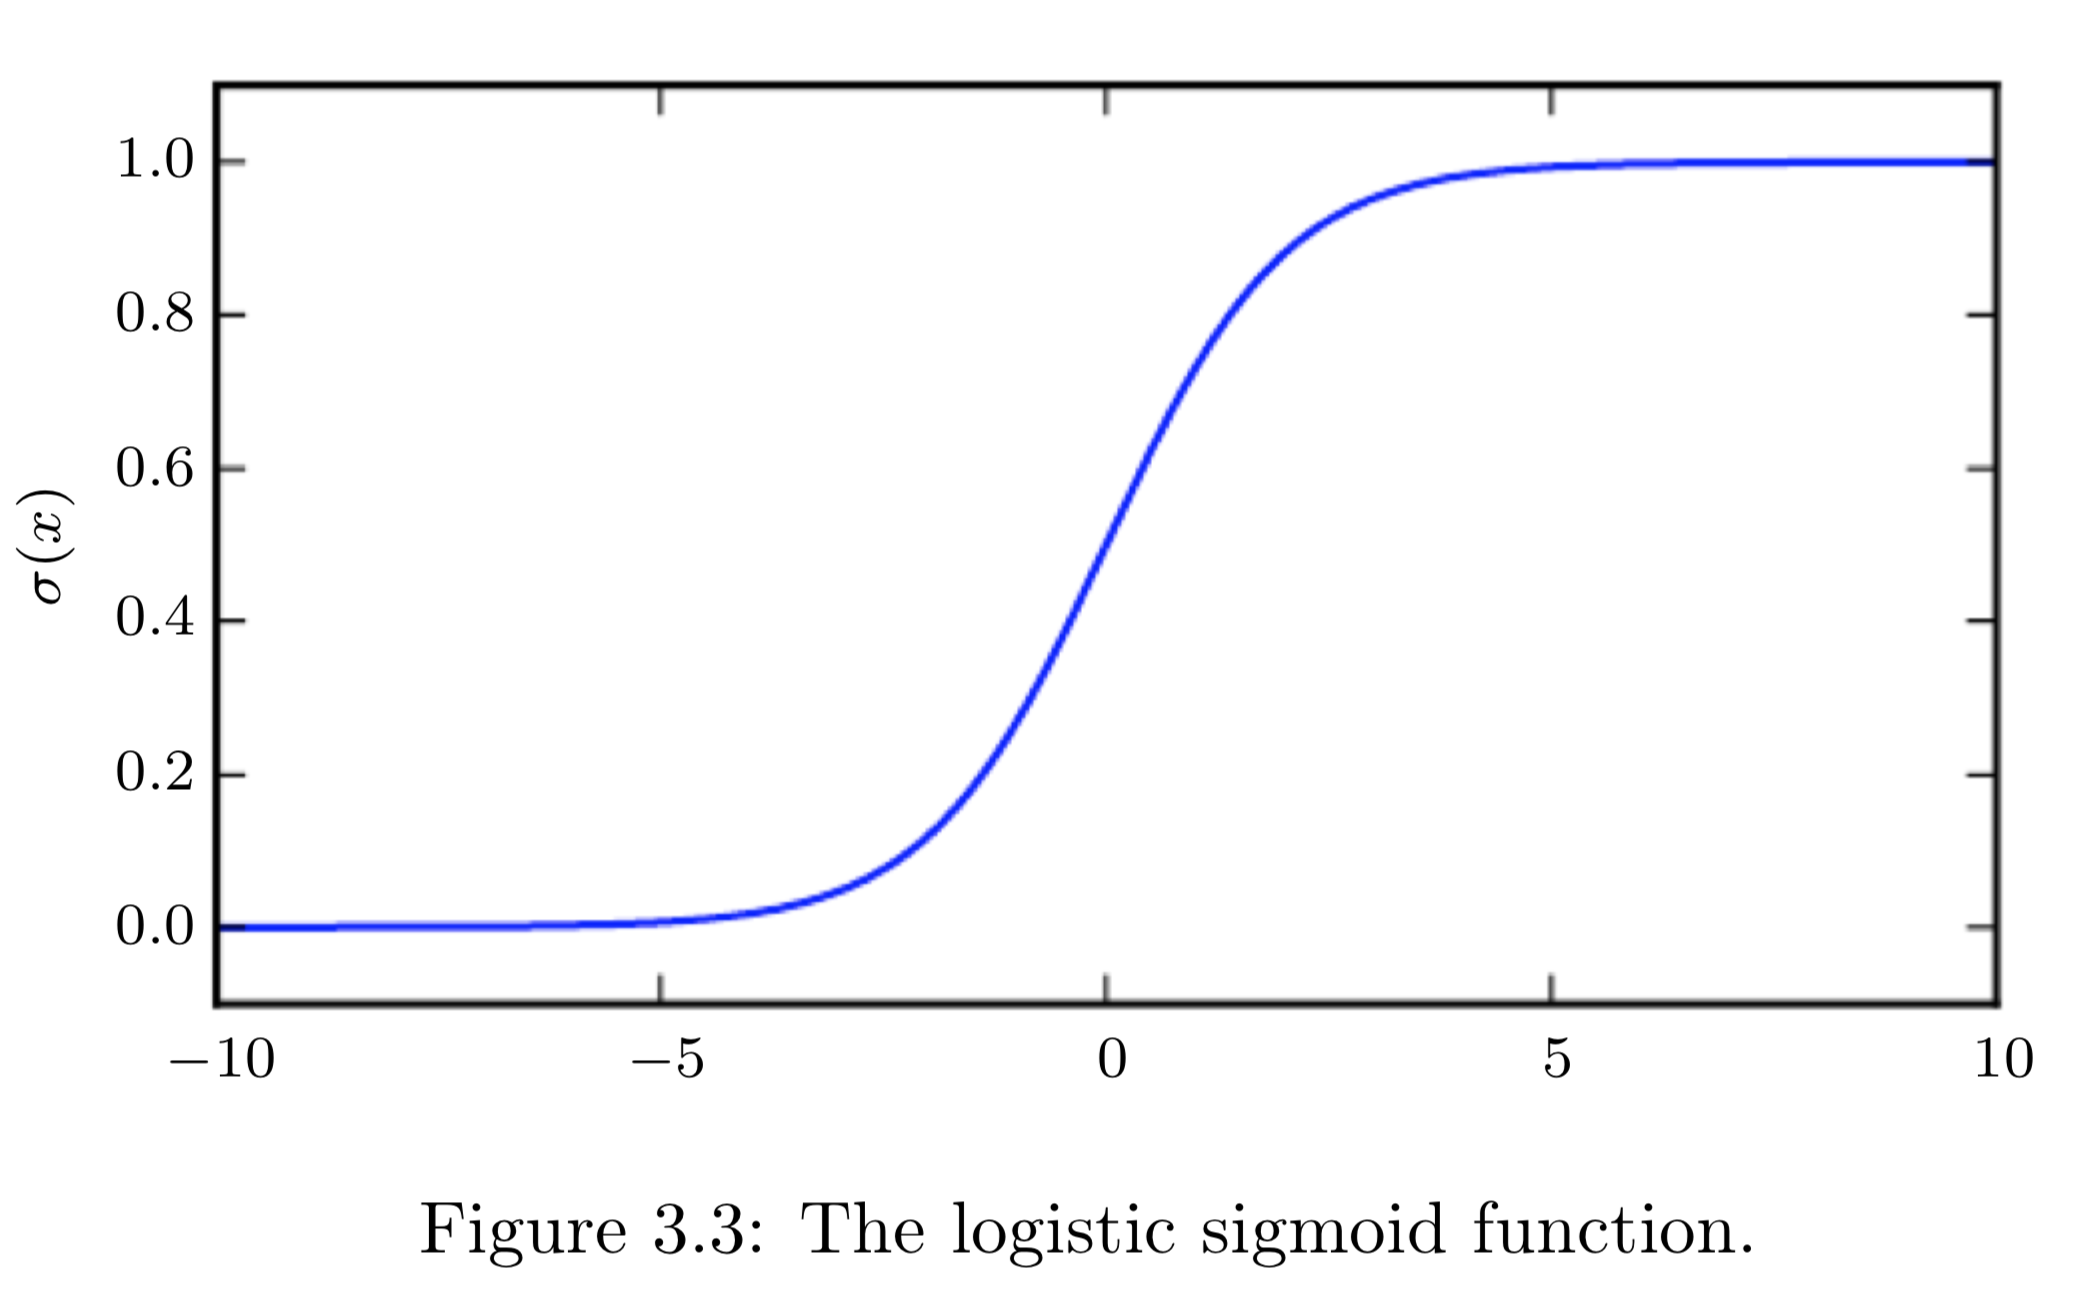
\includegraphics[scale=0.20]{images/3-3-sigmoid.png}
        \label{fig:3_3sigmoid}
        \caption{\textbf{sigmoid function}}
    \end{figure}
\end{frame}

\begin{frame}{3.10 Useful Properties of Common Functions}
    \justifying
    Another commonly encountered function is the \textbf{softplus} function (Dugas et al., 2001):
    \begin{equation}
        \zeta(x) = \log(1 + \exp(x)).
        \label{eq:3_31}
    \end{equation}
    
    The softplus function can be useful for producing the $\beta$ or $\sigma$ parameter of a normal distribution because its range is $(0, \infty)$. It also arises commonly when manipulating expressions involving sigmoids. The name of the softplus function comes from the fact that it is a smoothed or ``softened'' version of
    \begin{equation}
        x^{+} = \max\{0, x\}.
        \label{eq:3_32}
    \end{equation}
    
    See figure~3.4(\ref{fig:3_4softplus}) for a graph of the softplus function.
\end{frame}

\begin{frame}{3.10 Useful Properties of Common Functions}
    \begin{figure}
        \centering
        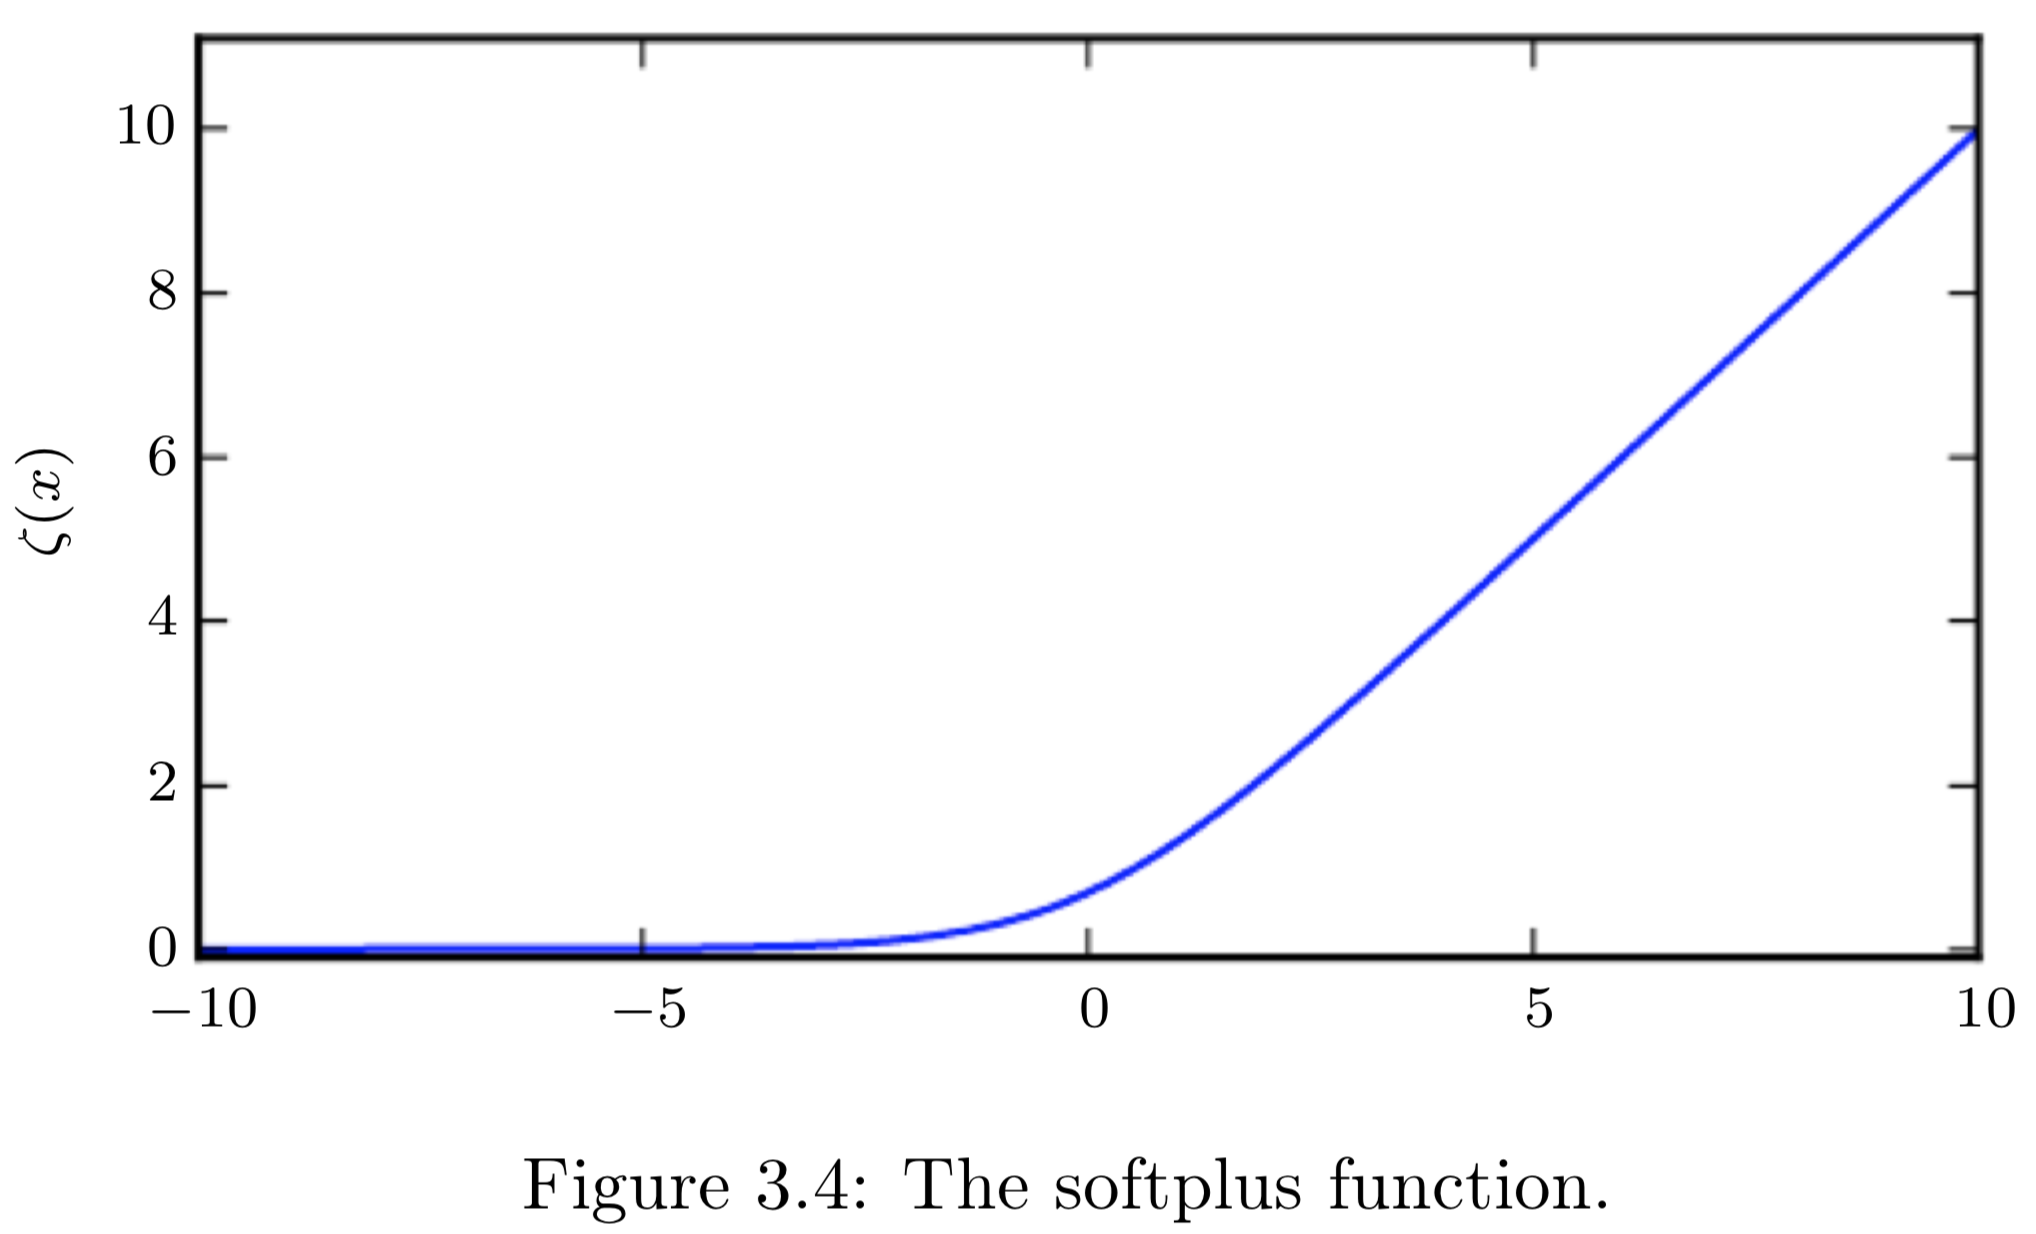
\includegraphics[scale=0.20]{images/3-4-softplus.png}
        \label{fig:3_4softplus}
        \caption{\textbf{softplus function}}
    \end{figure}
\end{frame}

\begin{frame}{3.10 Useful Properties of Common Functions}
    \justifying
    The following properties are all useful enough that you may wish to memorize them:
    \begin{align}
        \sigma(x) &= \frac{\exp(x)}{\exp(x) + \exp(0)} \label{eq:3_33} \\
        \frac{d}{dx}\left(\sigma(x)\right) &= \sigma(x)(1 - \sigma(x)) \label{eq:3_34} \\
        1 - \sigma(x) &= \sigma(-x) \label{eq:3_35} \\
        \log(\sigma(x)) &= -\zeta(-x) \label{eq:3_36}
    \end{align}
\end{frame}

\begin{frame}{3.10 Useful Properties of Common Functions}
    \begin{align}
        \frac{d}{dx}\left(\zeta(x)\right) &= \sigma(x) \label{eq:3_37} \\
        \forall x \in (0, 1), \sigma^{-1}(x) &= \log\left(\frac{x}{1 - x}\right) \label{eq:3_38} \\
        \forall x > 0, \zeta^{-1}(x) &= \log(\exp(x) - 1) \label{eq:3_39} \\
        \zeta(x) &= \int^{x}_{-\infty}\sigma(y)dy \label{eq:3_40} \\
        \zeta(x) - \zeta(-x) & = x \label{eq:3_41}
    \end{align}
    
    The function $\sigma^{-1}(x)$ is called the \textbf{logit} in statistics, but this term is more rarely used in machine learning.
\end{frame}

\begin{frame}{3.10 Useful Properties of Common Functions}
    \justifying
    Equation~\ref{eq:3_41} provides extra justification for the name ``softplus''. The softplus function is intended as a smoothed version of the \textbf{positive part} function, $x^{+} = \max\{0, x\}$. The positive part function is the counterpart of the \textbf{negative part} function, $x^{-} = \max\{0, -x\}$. To obtain a smooth function that is analogous to the negative part, one can use $\zeta(-x)$. Just as $x$ can be recovered from its positive part and negative part via the identity $x^{+} - x^{-} = x$, it is also possible to recover $x$ using the same relationship between $\zeta(x)$ and $\zeta(-x)$, as shown in equation~\ref{eq:3_41}.
\end{frame}

% ======================================= Bayes' Rule
\subsection{Bayes' Rule}
\begin{frame}{3.11 Bayes' Rule}
    \justifying
    We often find ourselves in a situation where we know $P(\mathrm{y} | \mathrm{x})$ and need to know $P(\mathrm{x} | \mathrm{y})$. Fortunately, if we also know $P(\mathrm{x})$, we can compute the desired quantity using \textbf{Bayes’ rule}:
    \begin{equation}
        P(\mathrm{x} | \mathrm{y}) = \frac{P(\mathrm{x}) P(\mathrm{y} | \mathrm{x})}{P(\mathrm{y})}.
        \label{eq:3_42}
    \end{equation}
\end{frame}

\begin{frame}{3.11 Bayes' Rule}
    \justifying   
    Note that while $P(\mathrm{y})$ appears in the formula, it is usually feasible to compute $P(\mathrm{y}) = \sum_{x} P(\mathrm{y} | x) P(x)$, so we do not need to begin with knowledge of $P(\mathrm{y})$.
    
    Bayes’ rule is straightforward to derive from the definition of conditional probability, but it is useful to know the name of this formula since many texts refer to it by name. It is named after the Reverend Thomas Bayes, who first discovered a special case of the formula. The general version presented here was independently discovered by Pierre-Simon Laplace.
\end{frame}

% ======================================= Technical Details of Continuous Variables
\subsection{Technical Details of Continuous Variables}
\begin{frame}{3.12 Technical Details of Continuous Variables}
    \justifying
    A proper formal understanding of continuous random variables and probability density functions requires developing probability theory in terms of a branch of mathematics known as measure theory. Measure theory is beyond the scope of this textbook, but we can briefly sketch some of the issues that measure theory is employed to resolve.
\end{frame}

\begin{frame}{3.12 Technical Details of Continuous Variables}
    \justifying   
    In section 3.3.2, we saw that the probability of a continuous vector-valued $\boldsymbol{\mathrm{x}}$ lying in some set $\mathbb{S}$ is given by the integral of $p(\boldsymbol{x})$ over the set $\mathbb{S}$. Some choices of set $\mathbb{S}$ can produce paradoxes. For example, it is possible to construct two sets $\mathbb{S}_{1}$ and $\mathbb{S}_{2}$ such that $p(\boldsymbol{x} \in \mathbb{S}_{1}) + p(\boldsymbol{x} \in \mathbb{S}_{2}) > 1$ but $\mathbb{S}_{1} \cap \mathbb{S}_{2} = \emptyset$. These sets are generally constructed making very heavy use of the infinite precision of real numbers, for example by making fractal-shaped sets or sets that are defined by transforming the set of rational numbers (tem nota de rodap\'{e} aqui). One of the key contributions of measure theory is to provide a characterization of the set of sets that we can compute the probability of without encountering paradoxes. In this book, we only integrate over sets with relatively simple descriptions, so this aspect of measure theory never becomes a relevant concern.
\end{frame}

\begin{frame}{3.12 Technical Details of Continuous Variables}
    \justifying
    For our purposes, measure theory is more useful for describing theorems that apply to most points in $\mathbb{R}^{n}$ but do not apply to some corner cases. Measure theory provides a rigorous way of describing that a set of points is negligibly small. Such a set is said to have \textbf{measure zero}. We do not formally define this concept in this textbook. For our purposes, it is sufficient to understand the intuition that a set of measure zero occupies no volume in the space we are measuring. For example, within $\mathbb{R}^{2}$, a line has measure zero, while a filled polygon has positive measure. Likewise, an individual point has measure zero. Any union of countably many sets that each have measure zero also has measure zero (so the set of all the rational numbers has measure zero, for instance).
\end{frame}

\begin{frame}{3.12 Technical Details of Continuous Variables}
    \justifying
    Another useful term from measure theory is almost everywhere. A property that holds almost everywhere holds throughout all of space except for on a set of measure zero. Because the exceptions occupy a negligible amount of space, they can be safely ignored for many applications. Some important results in probability theory hold for all discrete values but only hold ``almost everywhere'' for continuous values.
\end{frame}

\begin{frame}{3.12 Technical Details of Continuous Variables}
    \justifying
    Another technical detail of continuous variables relates to handling continuous random variables that are deterministic functions of one another. Suppose we have two random variables, $\boldsymbol{\mathrm{x}}$ and $\boldsymbol{\mathrm{y}}$, such that $\boldsymbol{y} = g(\boldsymbol{x})$, where $g$ is an invertible, continuous, differentiable transformation. One might expect that $p_{y}(\boldsymbol{y}) = p_{x}(g^{-1}(\boldsymbol{y}))$. This is actually not the case.
\end{frame}

\begin{frame}{3.12 Technical Details of Continuous Variables}
    \justifying
    As a simple example, suppose we have scalar random variables $\mathrm{x}$ and $\mathrm{y}$. Suppose $\mathrm{y} = \frac{\mathrm{x}}{2}$ and $\mathrm{x} \sim U(0, 1)$. If we use the rule $p_{y}(y) = p_{x}(2y)$ then $p_{y}$ will be $0$ everywhere except the interval $[0, \frac{1}{2}]$ , and it will be $1$ on this interval. This means
    \begin{equation}
        \int p_{y}(y)dy = \frac{1}{2},
        \label{eq:3_43}
    \end{equation}
    which violates the definition of a probability distribution. This is a common mistake. The problem with this approach is that it fails to account for the distortion of space introduced by the function $g$. Recall that the probability of $\boldsymbol{x}$ lying in an infinitesimally small region with volume $\delta\boldsymbol{x}$ is given by $p(\boldsymbol{x})\delta\boldsymbol{x}$. Since $g$ can expand or contract space, the infinitesimal volume surrounding $\boldsymbol{x}$ in $\boldsymbol{x}$ space may have different volume in $\boldsymbol{y}$ space.
\end{frame}

\begin{frame}{3.12 Technical Details of Continuous Variables}
    \justifying
    To see how to correct the problem, we return to the scalar case. We need to preserve the property
    \begin{equation}
        |p_{y}(g(x))dy| = |p_{x}(x)dx|.
        \label{eq:3_44}
    \end{equation}
    Solving from this, we obtain
    \begin{equation}
        p_{y}(y) = p_{x}(g^{-1}(y))\left|\frac{\partial x}{\partial y}\right|
        \label{eq:3_45}
    \end{equation}
    or equivalently
    \begin{equation}
        p_{x}(x) = p_{y}(g(x))\left|\frac{\partial g(x)}{\partial x}\right|.
        \label{eq:3_46}
    \end{equation}
\end{frame}

\begin{frame}{3.12 Technical Details of Continuous Variables}
    \justifying
    In higher dimensions, the derivative generalizes to the determinant of the \textbf{Jacobian matrix} -- the matrix with $J_{i,j} = \frac{\partial x_{i}}{\partial y_{j}}$. Thus, for real-valued vectors $\boldsymbol{x}$ and $\boldsymbol{y}$,
    \begin{equation}
        p_{x}(\boldsymbol{x}) = p_{y}(g(\boldsymbol{x}))\left|\det{\left(\frac{\partial g(\boldsymbol{x})}{\partial \boldsymbol{x}} \right)}\right|.
        \label{eq:3_47}
    \end{equation}
\end{frame}

% ======================================= Information Theory
\subsection{Information Theory}
\begin{frame}{3.13 Information Theory}
    \justifying
    Information theory is a branch of applied mathematics that revolves around quantifying how much information is present in a signal. It was originally invented to study sending messages from discrete alphabets over a noisy channel, such as communication via radio transmission. In this context, information theory tells how to design optimal codes and calculate the expected length of messages sampled from specific probability distributions using various encoding schemes. In the context of machine learning, we can also apply information theory to continuous variables where some of these message length interpretations do not apply. This field is fundamental to many areas of electrical engineering and computer science. In this textbook, we mostly use a few key ideas from information theory to characterize probability distributions or quantify similarity between probability distributions. For more detail on information theory, see Cover and Thomas (2006) or MacKay (2003).
\end{frame}

\begin{frame}{3.13 Information Theory}
    \justifying
    The basic intuition behind information theory is that learning that an unlikely event has occurred is more informative than learning that a likely event has occurred. A message saying ``the sun rose this morning'' is so uninformative as to be unnecessary to send, but a message saying ``there was a solar eclipse this morning'' is very informative.
\end{frame}

\begin{frame}{3.13 Information Theory}
    \justifying
    We would like to quantify information in a way that formalizes this intuition. Specifically,
    \begin{itemize}
        \justifying
        \item Likely events should have low information content, and in the extreme case, events that are guaranteed to happen should have no information content whatsoever.
        \item Less likely events should have higher information content.
        \item Independent events should have additive information. For example, finding out that a tossed coin has come up as heads twice should convey twice as much information as finding out that a tossed coin has come up as heads once.   
    \end{itemize}
\end{frame}

\begin{frame}{3.13 Information Theory}
    \justifying
    In order to satisfy all three of these properties, we define the self-information of an event $\mathrm{x} = x$ to be
    \begin{equation}
        I(x) = -\log{P(x)}.
        \label{eq:3_48}
    \end{equation}
    In this book, we always use $\log$ to mean the natural logarithm, with base $e$. Our definition of $I(x)$ is therefore written in units of \textbf{nats}. One nat is the amount of information gained by observing an event of probability $\frac{1}{e}$. Other texts use base-2 logarithms and units called \textbf{bits} or \textbf{shannons}; information measured in bits is just a rescaling of information measured in nats.
\end{frame}

\begin{frame}{3.13 Information Theory}
    \justifying
    When $\mathrm{x}$ is continuous, we use the same definition of information by analogy, but some of the properties from the discrete case are lost. For example, an event with unit density still has zero information, despite not being an event that is guaranteed to occur.
    
    Self-information deals only with a single outcome. We can quantify the amount of uncertainty in an entire probability distribution using the \textbf{Shannon entropy}: 
    \begin{equation}
        H(\mathrm{x}) = \mathbb{E}_{\mathrm{x} \sim P}[I(x)] = -\mathbb{E}_{\mathrm{x} \sim P}[\log{P(x)}],
        \label{eq:3_49}
    \end{equation}
    also denoted $H(P)$.
\end{frame}

\begin{frame}{3.13 Information Theory}
    \justifying
    In other words, the Shannon entropy of a distribution is the expected amount of information in an event drawn from that distribution. It gives a lower bound on the number of bits (if the logarithm is base $2$, otherwise the units are different) needed on average to encode symbols drawn from a distribution $P$. Distributions that are nearly deterministic (where the outcome is nearly certain) have low entropy; distributions that are closer to uniform have high entropy. See figure 3.5~(\ref{fig:3_5shannon}) for a demonstration. When $\mathrm{x}$ is continuous, the Shannon entropy is known as the \textbf{differential entropy}.
\end{frame}

\begin{frame}{3.13 Information Theory}
    \begin{figure}
        \centering
        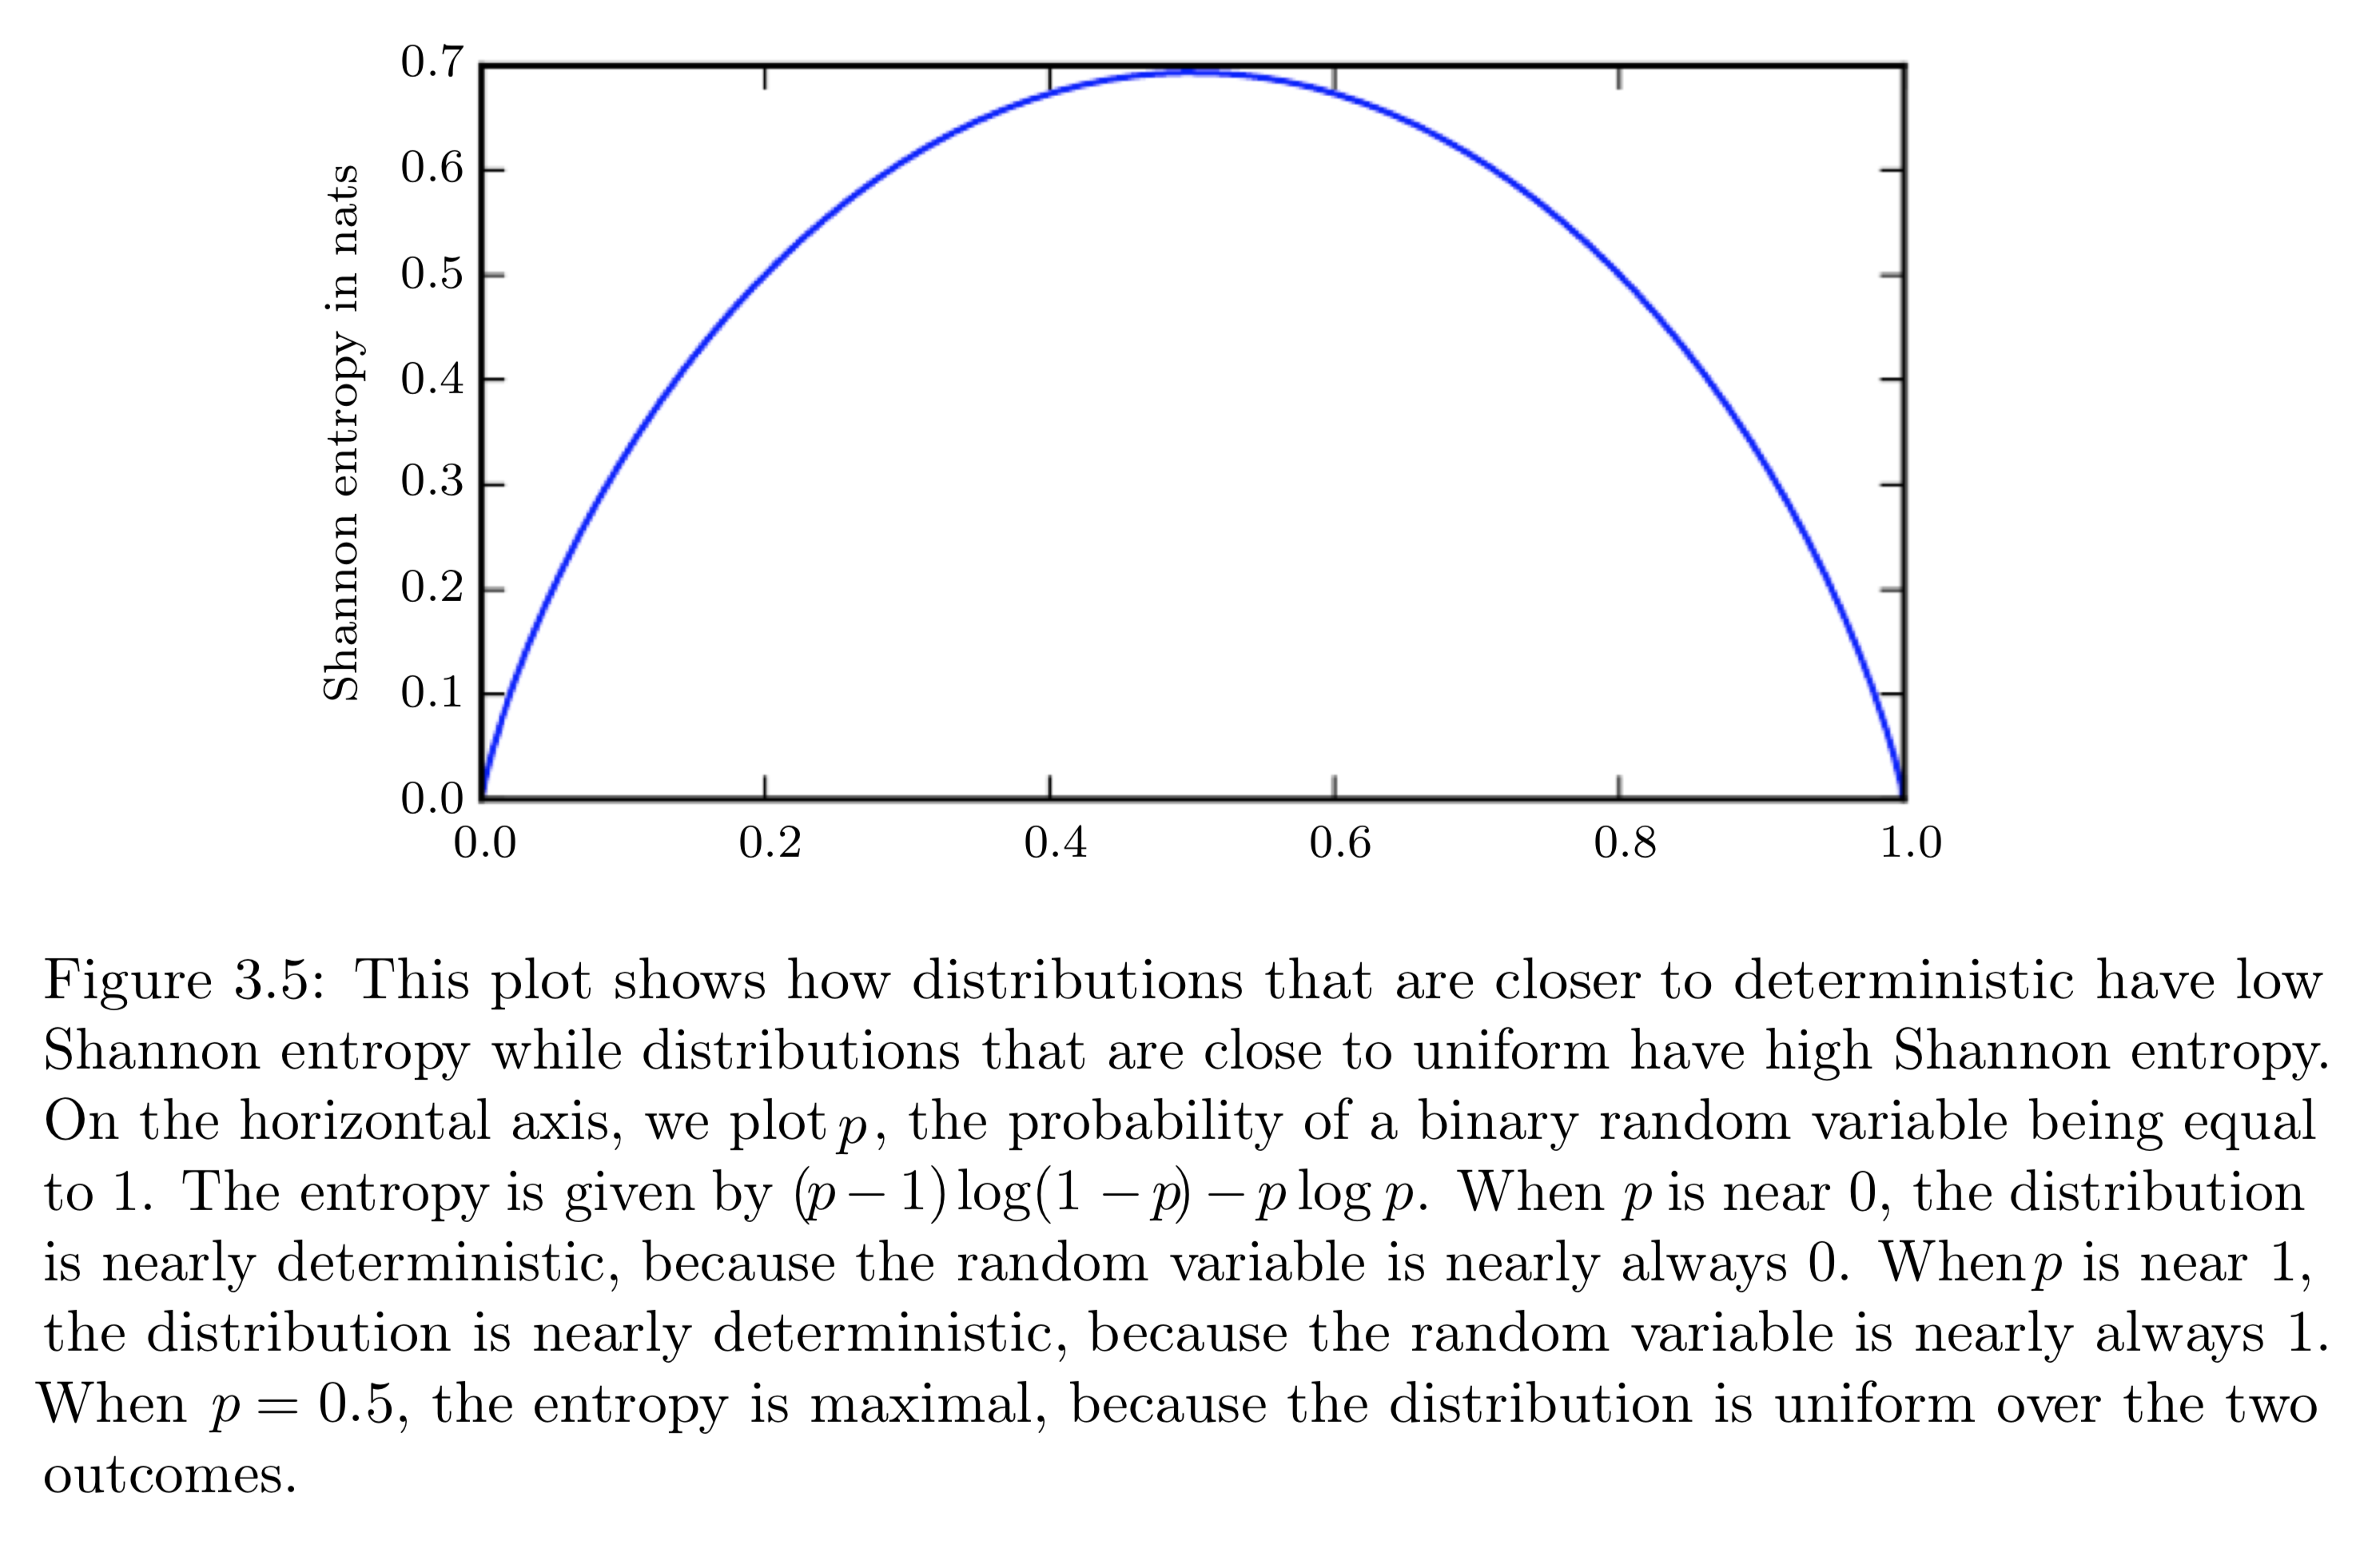
\includegraphics[scale=0.20]{images/3-5-shannon.png}
        \label{fig:3_5shannon}
        \caption{\textbf{Shannon}}
    \end{figure}
\end{frame}

\begin{frame}{3.13 Information Theory}
    \justifying
    If we have two separate probability distributions P (x) and Q (x) over the same random variable x, we can measure how different these two distributions are using the Kullback-Leibler (KL) divergence:
    \begin{align}
        D_{KL}(P||Q) &= \mathbb{E}_{\mathrm{x} \sim P} \left[\log\left(\frac{P(x)}{Q(x)}\right) \right] \nonumber\\
                     &= \mathbb{E}_{\mathrm{x} \sim P}[\log(P(x)) - \log(Q(x))].
        \label{qe:3_50}
    \end{align}
\end{frame}

\begin{frame}{3.13 Information Theory}
    \justifying
    In the case of discrete variables, it is the extra amount of information (measured in bits if we use the base $2$ logarithm, but in machine learning we usually use nats and the natural logarithm) needed to send a message containing symbols drawn from probability distribution $P$, when we use a code that was designed to minimize the length of messages drawn from probability distribution $Q$.
\end{frame}

\begin{frame}{3.13 Information Theory}
    \justifying
    The $KL$ divergence has many useful properties, most notably that it is non-negative. The $KL$ divergence is $0$ if and only if $P$ and $Q$ are the same distribution in the case of discrete variables, or equal ``almost everywhere'' in the case of continuous variables. Because the $KL$ divergence is non-negative and measures the difference between two distributions, it is often conceptualized as measuring some sort of distance between these distributions. However, it is not a true distance measure because it is not symmetric: $D_{KL}(P||Q) \neq = D_{KL}(Q||P)$ for some $P$ and $Q$. This asymmetry means that there are important consequences to the choice of whether to use $D_{KL}(P||Q)$ or $D_{KL}(Q||P)$. See figure 3.6~(\ref{fig:3_6prob_KL}) for more detail.
\end{frame}

\begin{frame}{3.13 Information Theory}
    \begin{figure}
        \centering
        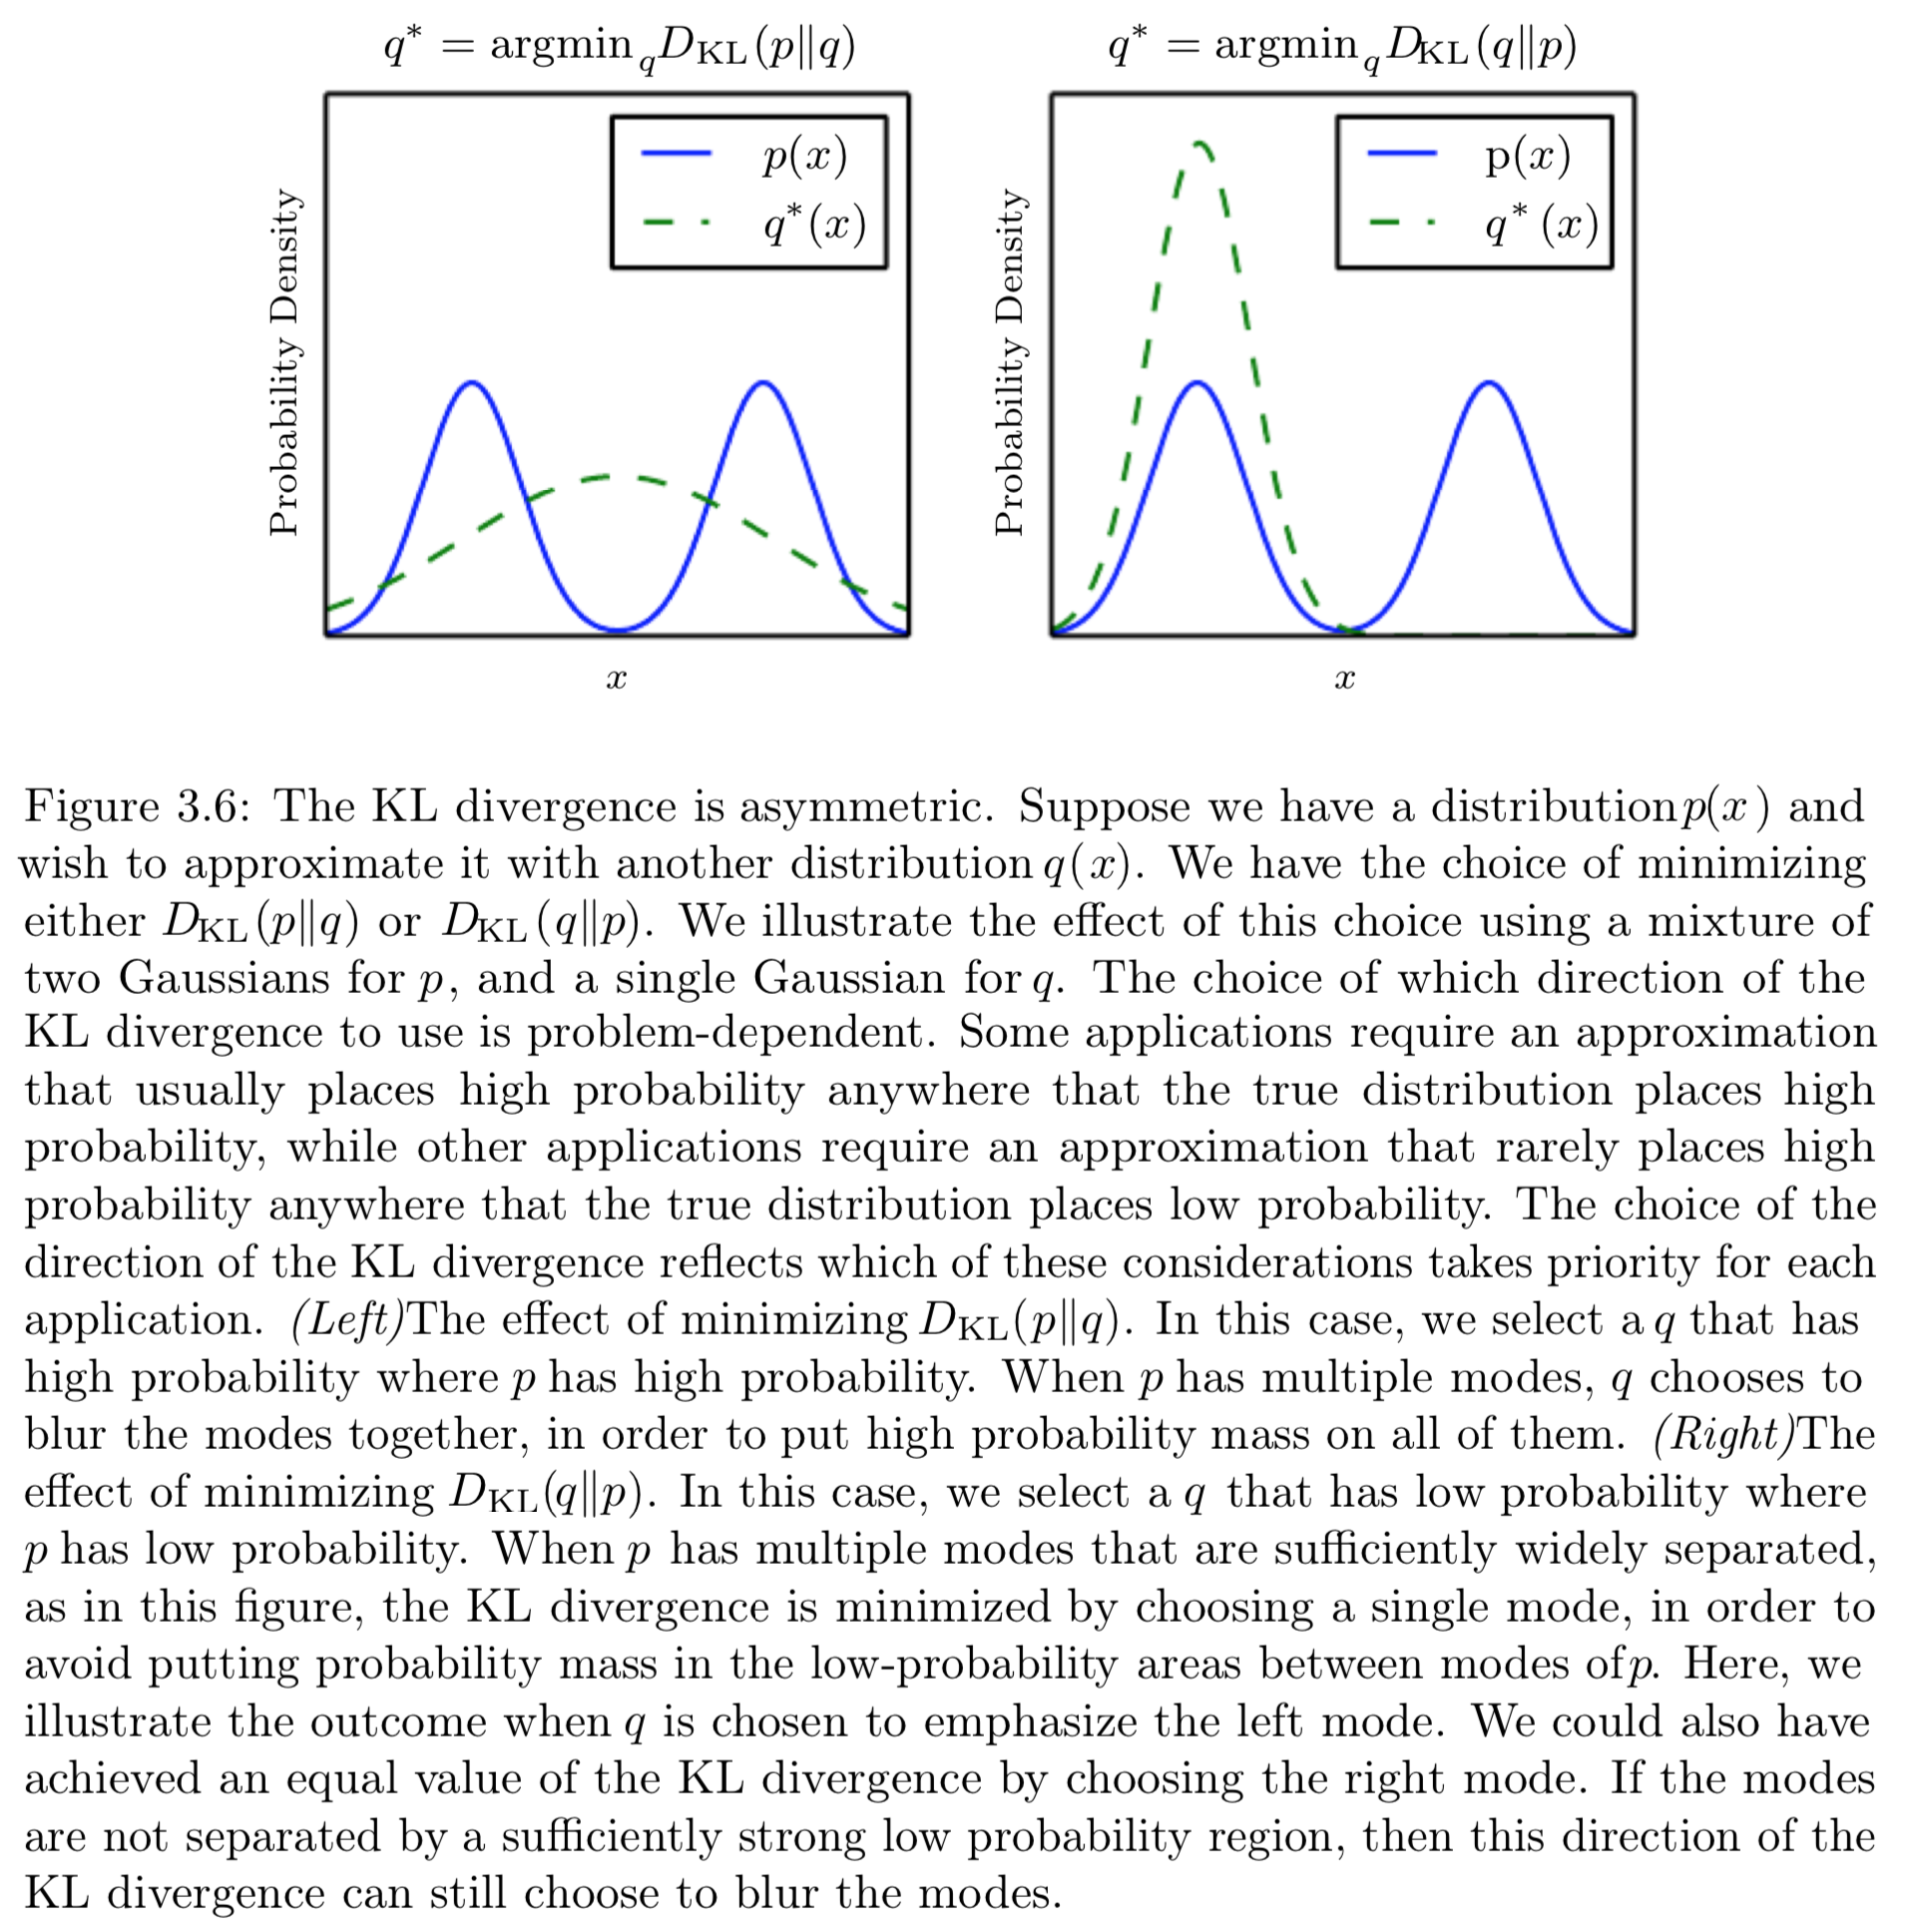
\includegraphics[scale=0.20]{images/3-6-prob_KL.png}
        \label{fig:3_6prob_KL}
        \caption{\textbf{KL}}
    \end{figure}
\end{frame}

\begin{frame}{3.13 Information Theory}
    \justifying
    A quantity that is closely related to the KL divergence is the cross-entropy H(P, Q) = H (P ) + D KL (P  Q ), which is similar to the KL divergence but lacking the term on the left:
    \begin{equation}
        H(P, Q) = -\mathbb{E}_{\mathrm{x} \sim P} \log(Q(x)).
        \label{eq:3_51}
    \end{equation}
    
    Minimizing the cross-entropy with respect to $Q$ is equivalent to minimizing the $KL$ divergence, because $Q$ does not participate in the omitted term. When computing many of these quantities, it is common to encounter expressions of the form $0 \log 0$. By convention, in the context of information theory, we treat these expressions as $\lim_{x \rightarrow 0} x \log x = 0$.
\end{frame}

% ======================================= Structured Probabilistic Models
\subsection{Structured Probabilistic Models}
\begin{frame}{3.14 Structured Probabilistic Models}
    \justifying
    Machine learning algorithms often involve probability distributions over a very large number of random variables. Often, these probability distributions involve direct interactions between relatively few variables. Using a single function to describe the entire joint probability distribution can be very inefficient (both computationally and statistically).
\end{frame}

\begin{frame}{3.14 Structured Probabilistic Models}
    \justifying
    Instead of using a single function to represent a probability distribution, we can split a probability distribution into many factors that we multiply together. For example, suppose we have three random variables: a, b and c. Suppose that a influences the value of b and b influences the value of c, but that a and c are independent given b. We can represent the probability distribution over all three variables as a product of probability distributions over two variables:
    \begin{equation}
        p(a, b, c) = p(a) p(b|a) p(c|b).
        \label{eq:3_52}
    \end{equation}
\end{frame}

\begin{frame}{3.14 Structured Probabilistic Models}
    \justifying
    These factorizations can greatly reduce the number of parameters needed to describe the distribution. Each factor uses a number of parameters that is exponential in the number of variables in the factor. This means that we can greatly reduce the cost of representing a distribution if we are able to find a factorization into distributions over fewer variables.
    
    We can describe these kinds of factorizations using graphs. Here we use the word ``graph'' in the sense of graph theory: a set of vertices that may be connected to each other with edges. When we represent the factorization of a probability distribution with a graph, we call it a \textbf{structured probabilistic model} or \textbf{graphical model}.
\end{frame}

\begin{frame}{3.14 Structured Probabilistic Models}
    \justifying
    There are two main kinds of structured probabilistic models: directed and undirected. Both kinds of graphical models use a graph $\mathcal{G}$ in which each node in the graph corresponds to a random variable, and an edge connecting two random variables means that the probability distribution is able to represent direct interactions between those two random variables.
\end{frame}

\begin{frame}{3.14 Structured Probabilistic Models}
    \justifying
    \textbf{Directed} models use graphs with directed edges, and they represent factorizations into conditional probability distributions, as in the example above. Specifically, a directed model contains one factor for every random variable $\mathrm{x}_{i}$ in the distribution, and that factor consists of the conditional distribution over $\mathrm{x}_{i}$ given the parents of $\mathrm{x}_{i}$, denoted $P_{a \mathcal{G}}(\mathrm{x}_{i})$:
    \begin{equation}
        p(\boldsymbol{\mathrm{x}} = \prod_{i}p(\mathrm{x}_{i} | P_{a \mathcal{G}}(\mathrm{x}_{i})).
    \end{equation}
    See figure 3.7~(\ref{fig:3_7graph1}) for an example of a directed graph and the factorization of probability distributions it represents.
\end{frame}

\begin{frame}{3.14 Structured Probabilistic Models}
    \begin{figure}
        \centering
        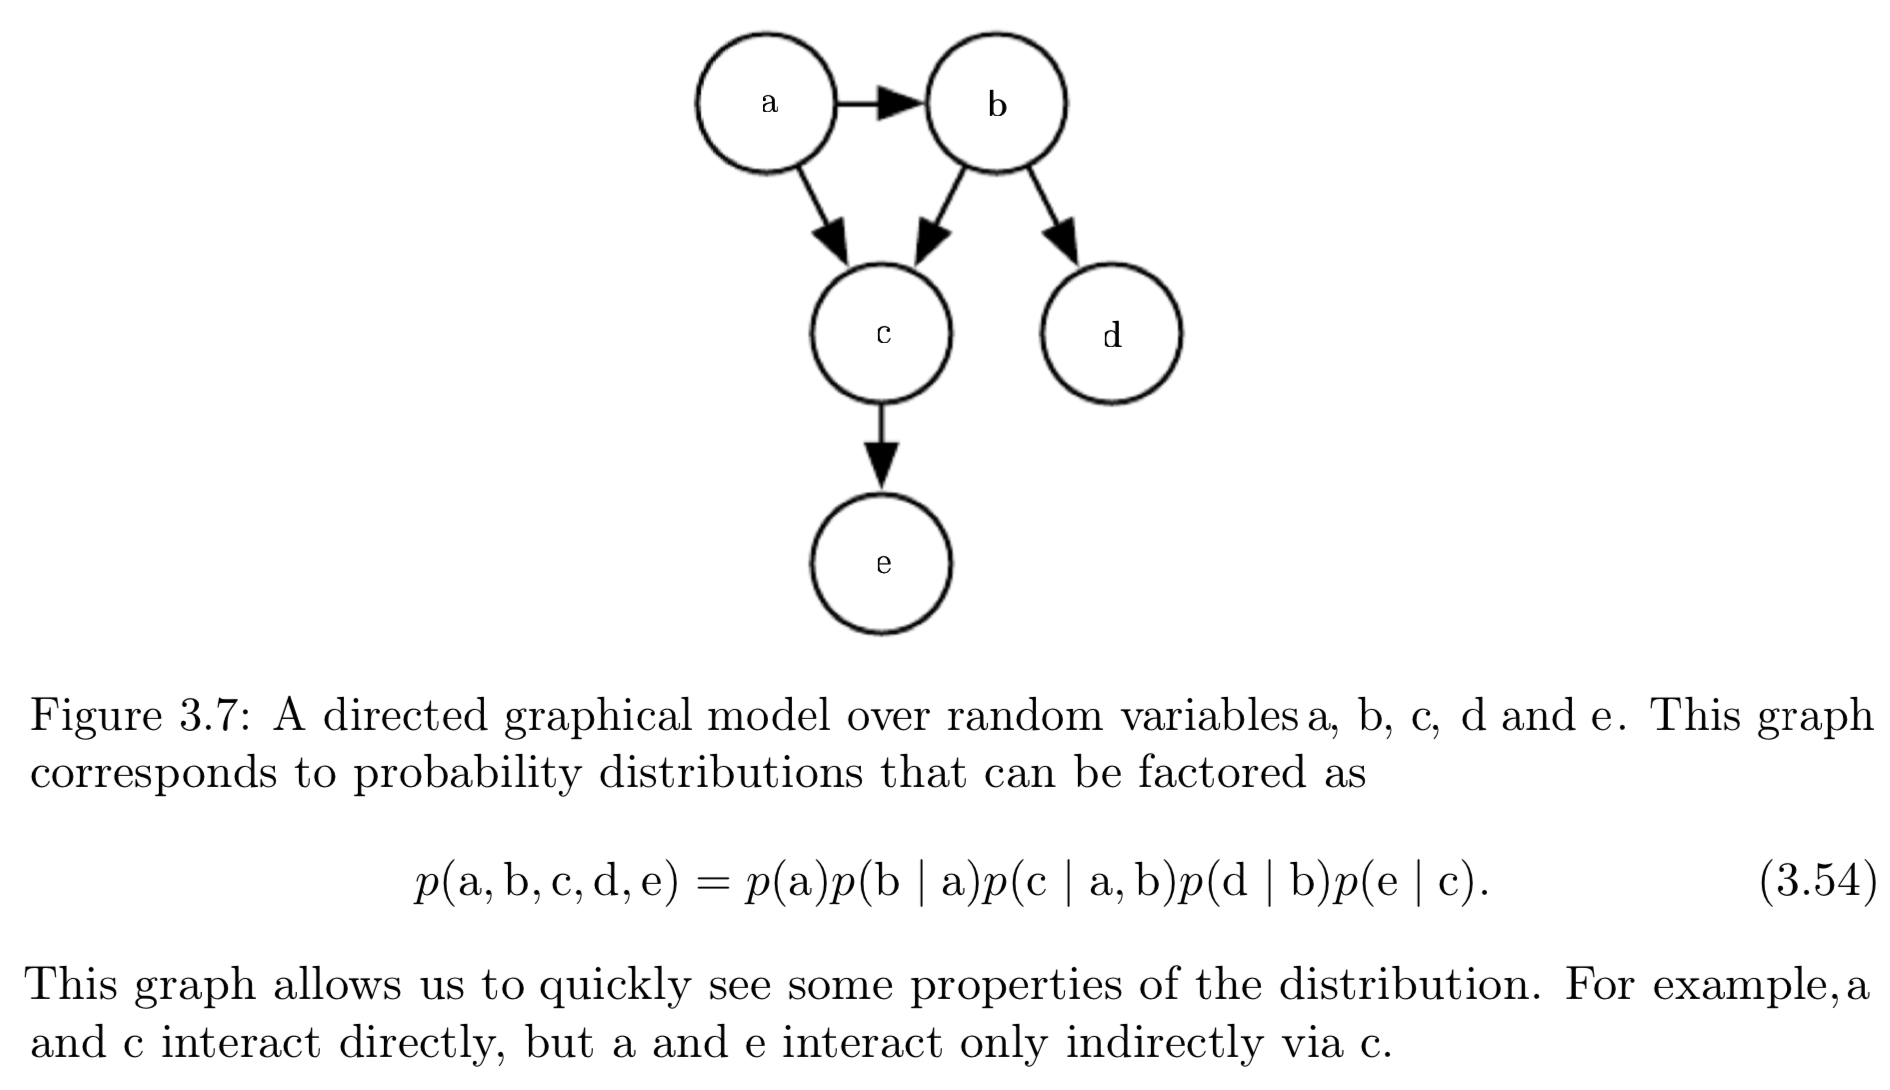
\includegraphics[scale=0.3]{images/3-7-graph_1.png}
        \label{fig:3_7graph1}
        \caption{\textbf{Graph Direct Model}}
    \end{figure}
\end{frame}

\begin{frame}{3.14 Structured Probabilistic Models}
    \justifying
    \textbf{Undirected} models use graphs with undirected edges, and they represent factorizations into a set of functions; unlike in the directed case, these functions are usually not probability distributions of any kind. Any set of nodes that are all connected to each other in $\mathcal{G}$ is called a clique. Each clique $\mathcal{C}^{(i)}$ in an undirected model is associated with a factor $\phi^{(i)}(\mathcal{C}^{(i)})$. These factors are just functions, not probability distributions. The output of each factor must be non-negative, but there is no constraint that the factor must sum or integrate to $1$ like a probability distribution.
\end{frame}

\begin{frame}{3.14 Structured Probabilistic Models}
    \justifying
    The probability of a configuration of random variables is \textbf{proportional} to the product of all of these factors -- assignments that result in larger factor values are more likely. Of course, there is no guarantee that this product will sum to $1$. We therefore divide by a normalizing constant $Z$, defined to be the sum or integral over all states of the product of the $\phi$ functions, in order to obtain a normalized probability distribution:
    \begin{equation}
        p(\boldsymbol{\mathrm{x}}) = \frac{1}{Z}\prod_{i}\phi^{(i)}\left(\mathcal{C}^{(i)}\right).
        \label{eq:3_55}
    \end{equation}
    
    See figure 3.8~(\ref{fig:3_8graph2}) for an example of an undirected graph and the factorization of probability distributions it represents.
\end{frame}

\begin{frame}{3.14 Structured Probabilistic Models}
    \begin{figure}
        \centering
        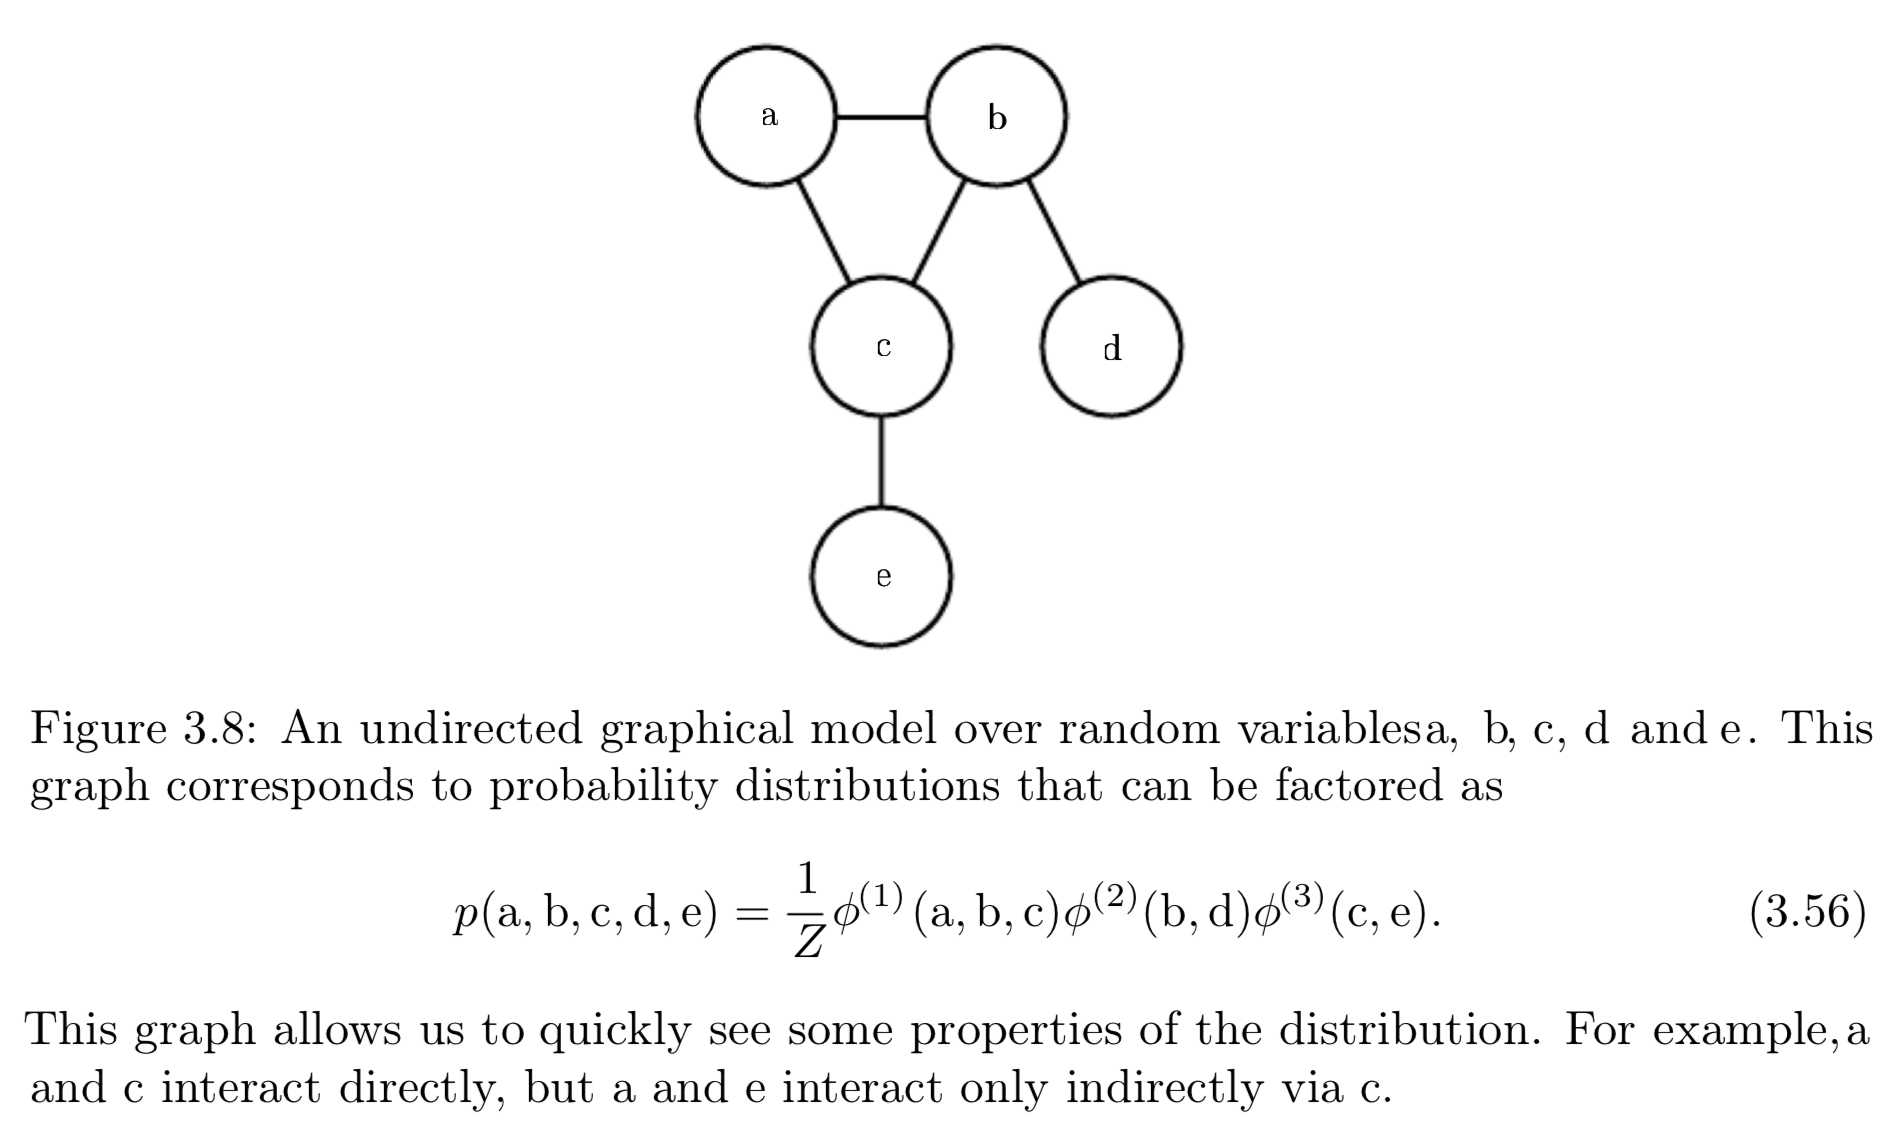
\includegraphics[scale=0.3]{images/3-8-graph_2.png}
        \label{fig:3_8graph2}
        \caption{\textbf{Graph Undirect Model}}
    \end{figure}
\end{frame}

\begin{frame}{3.14 Structured Probabilistic Models}
    \justifying
    Keep in mind that these graphical representations of factorizations are a language for describing probability distributions. They are not mutually exclusive families of probability distributions. Being directed or undirected is not a property of a probability distribution; it is a property of a particular \textbf{description} of a probability distribution, but any probability distribution may be described in both ways.
\end{frame}

\begin{frame}{3.14 Structured Probabilistic Models}
    \justifying
    Throughout parts I and II of this book, we will use structured probabilistic models merely as a language to describe which direct probabilistic relationships different machine learning algorithms choose to represent. No further understanding of structured probabilistic models is needed until the discussion of research topics, in part III , where we will explore structured probabilistic models in much greater detail.
    
    This chapter has reviewed the basic concepts of probability theory that are most relevant to deep learning. One more set of fundamental mathematical tools remains: numerical methods.
\end{frame}

